The clustering algorithms used for the SmartEater dataset, were DBSCAN and OPTICS. One of the advantages of these density-based clustering methods (as mentioned in section \ref{section:densityBasedMethods}) are that there are less parameters to configure. Another reason for choosing these methods, is that there is no need to define a fixed number of \textit{k} clusters to find, since the cluster boundaries are regulated by density. This technique also allows arbitrary-shaped clusters to be correctly identified. The t-SNE dimensionality reduction approach provided more significant results than PCA. Thus, the cleaned data and t-SNE modified data (with two components) was fed into the clustering algorithms DBSCAN and OPTICS.

\subsubsection{DBSCAN}
The DBSCAN algorithm was applied on the SmartEater dataset using the sklearn \textit{DBSCAN}\footnote{\url{https://scikit-learn.org/stable/modules/generated/sklearn.cluster.DBSCAN.html}} function.
Section \ref{section:DBSCAN} describes the functionality of the DBSCAN clustering method. As mentioned, one of the disadvantages of DBSCAN, is the need to specify parameters, which can change the outcome of the results. In order to establish suitable parameters, k-dist graphs were generated for the 1h and 3h datasets. The graphs contained the distances kth nearest neighbors. As recommended by \textcite{DBSCAN}[230], \textit{MinPts} and \textit{k} were set to 4 and the graphs were used to determine \textit{Eps}. The idea was to select \textit{Eps} suitable for the "thinnest" cluster, however being careful to avoid noise. As can be seen in figures \ref{figure:kDistGraphDBSCAN1h} and \ref{figure:kDistGraphDBSCAN3h}, the valley starts at roughly a 4th nearest neighbor distance of 2. 


\begin{figure}[H]
  \centering
  \begin{subfigure}{.5\textwidth}
    \centering
    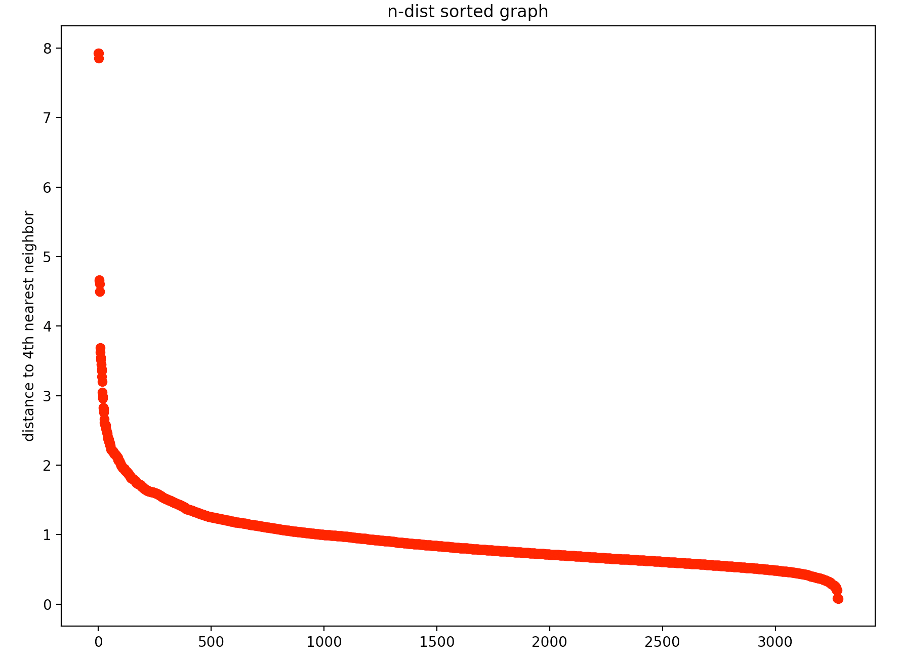
\includegraphics[width=0.87\textwidth]{./images/kDistGraphDBSCAN1h.png}
  \caption{1h dataset}
  \label{figure:kDistGraphDBSCAN1h}
  \end{subfigure}%
  \hfill
  \begin{subfigure}{.5\textwidth}
    \centering
    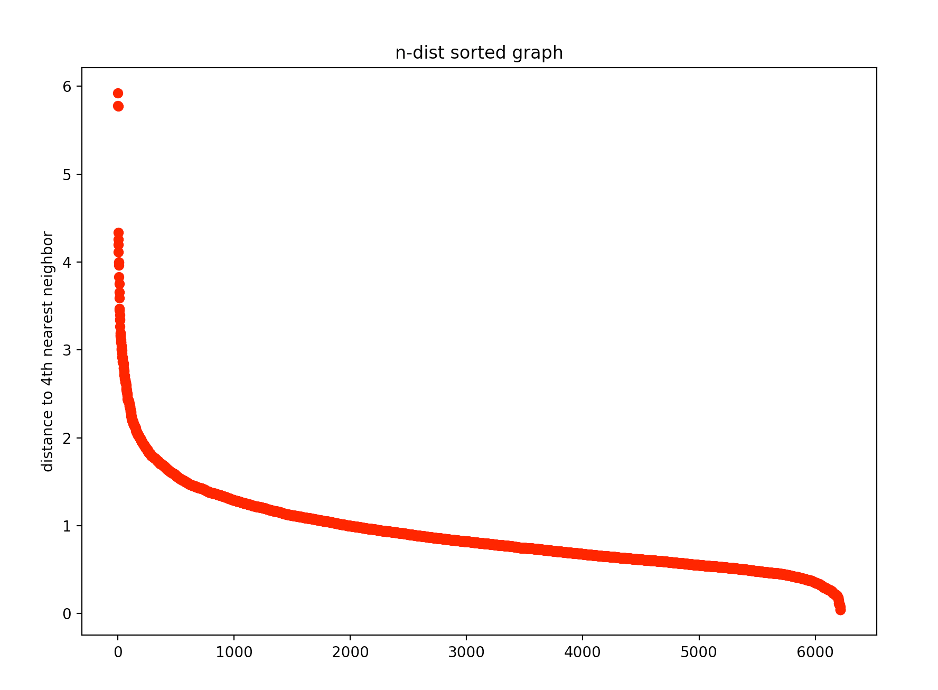
\includegraphics[width=1\textwidth]{./images/kDistGraphDBSCAN3h.png}
    \caption{3h dataset}
    \label{figure:kDistGraphDBSCAN3h}
  \end{subfigure}
  \caption{Sorted 4-dist graphs (distance for each point to its fourth nearest neighbor), used to determine a suitable Eps parameter for the DBSCAN algorithm. The valley starts at roughly the 4th nearest neighbor distance of 2, therefore Eps should be 2.}
  \label{figure:kDistGraphDBSCAN}
  \end{figure}

The DBSCAN algorithm was applied, with the parameters eps = 2 and min\_samples (MinPts) = 4. The results of this clustering method can be seen in figure \ref{figure:DBSCANResults}.


\begin{figure}[H]
  \centering
  \begin{subfigure}{.5\textwidth}\captionsetup{width=.8\linewidth}
    \centering
    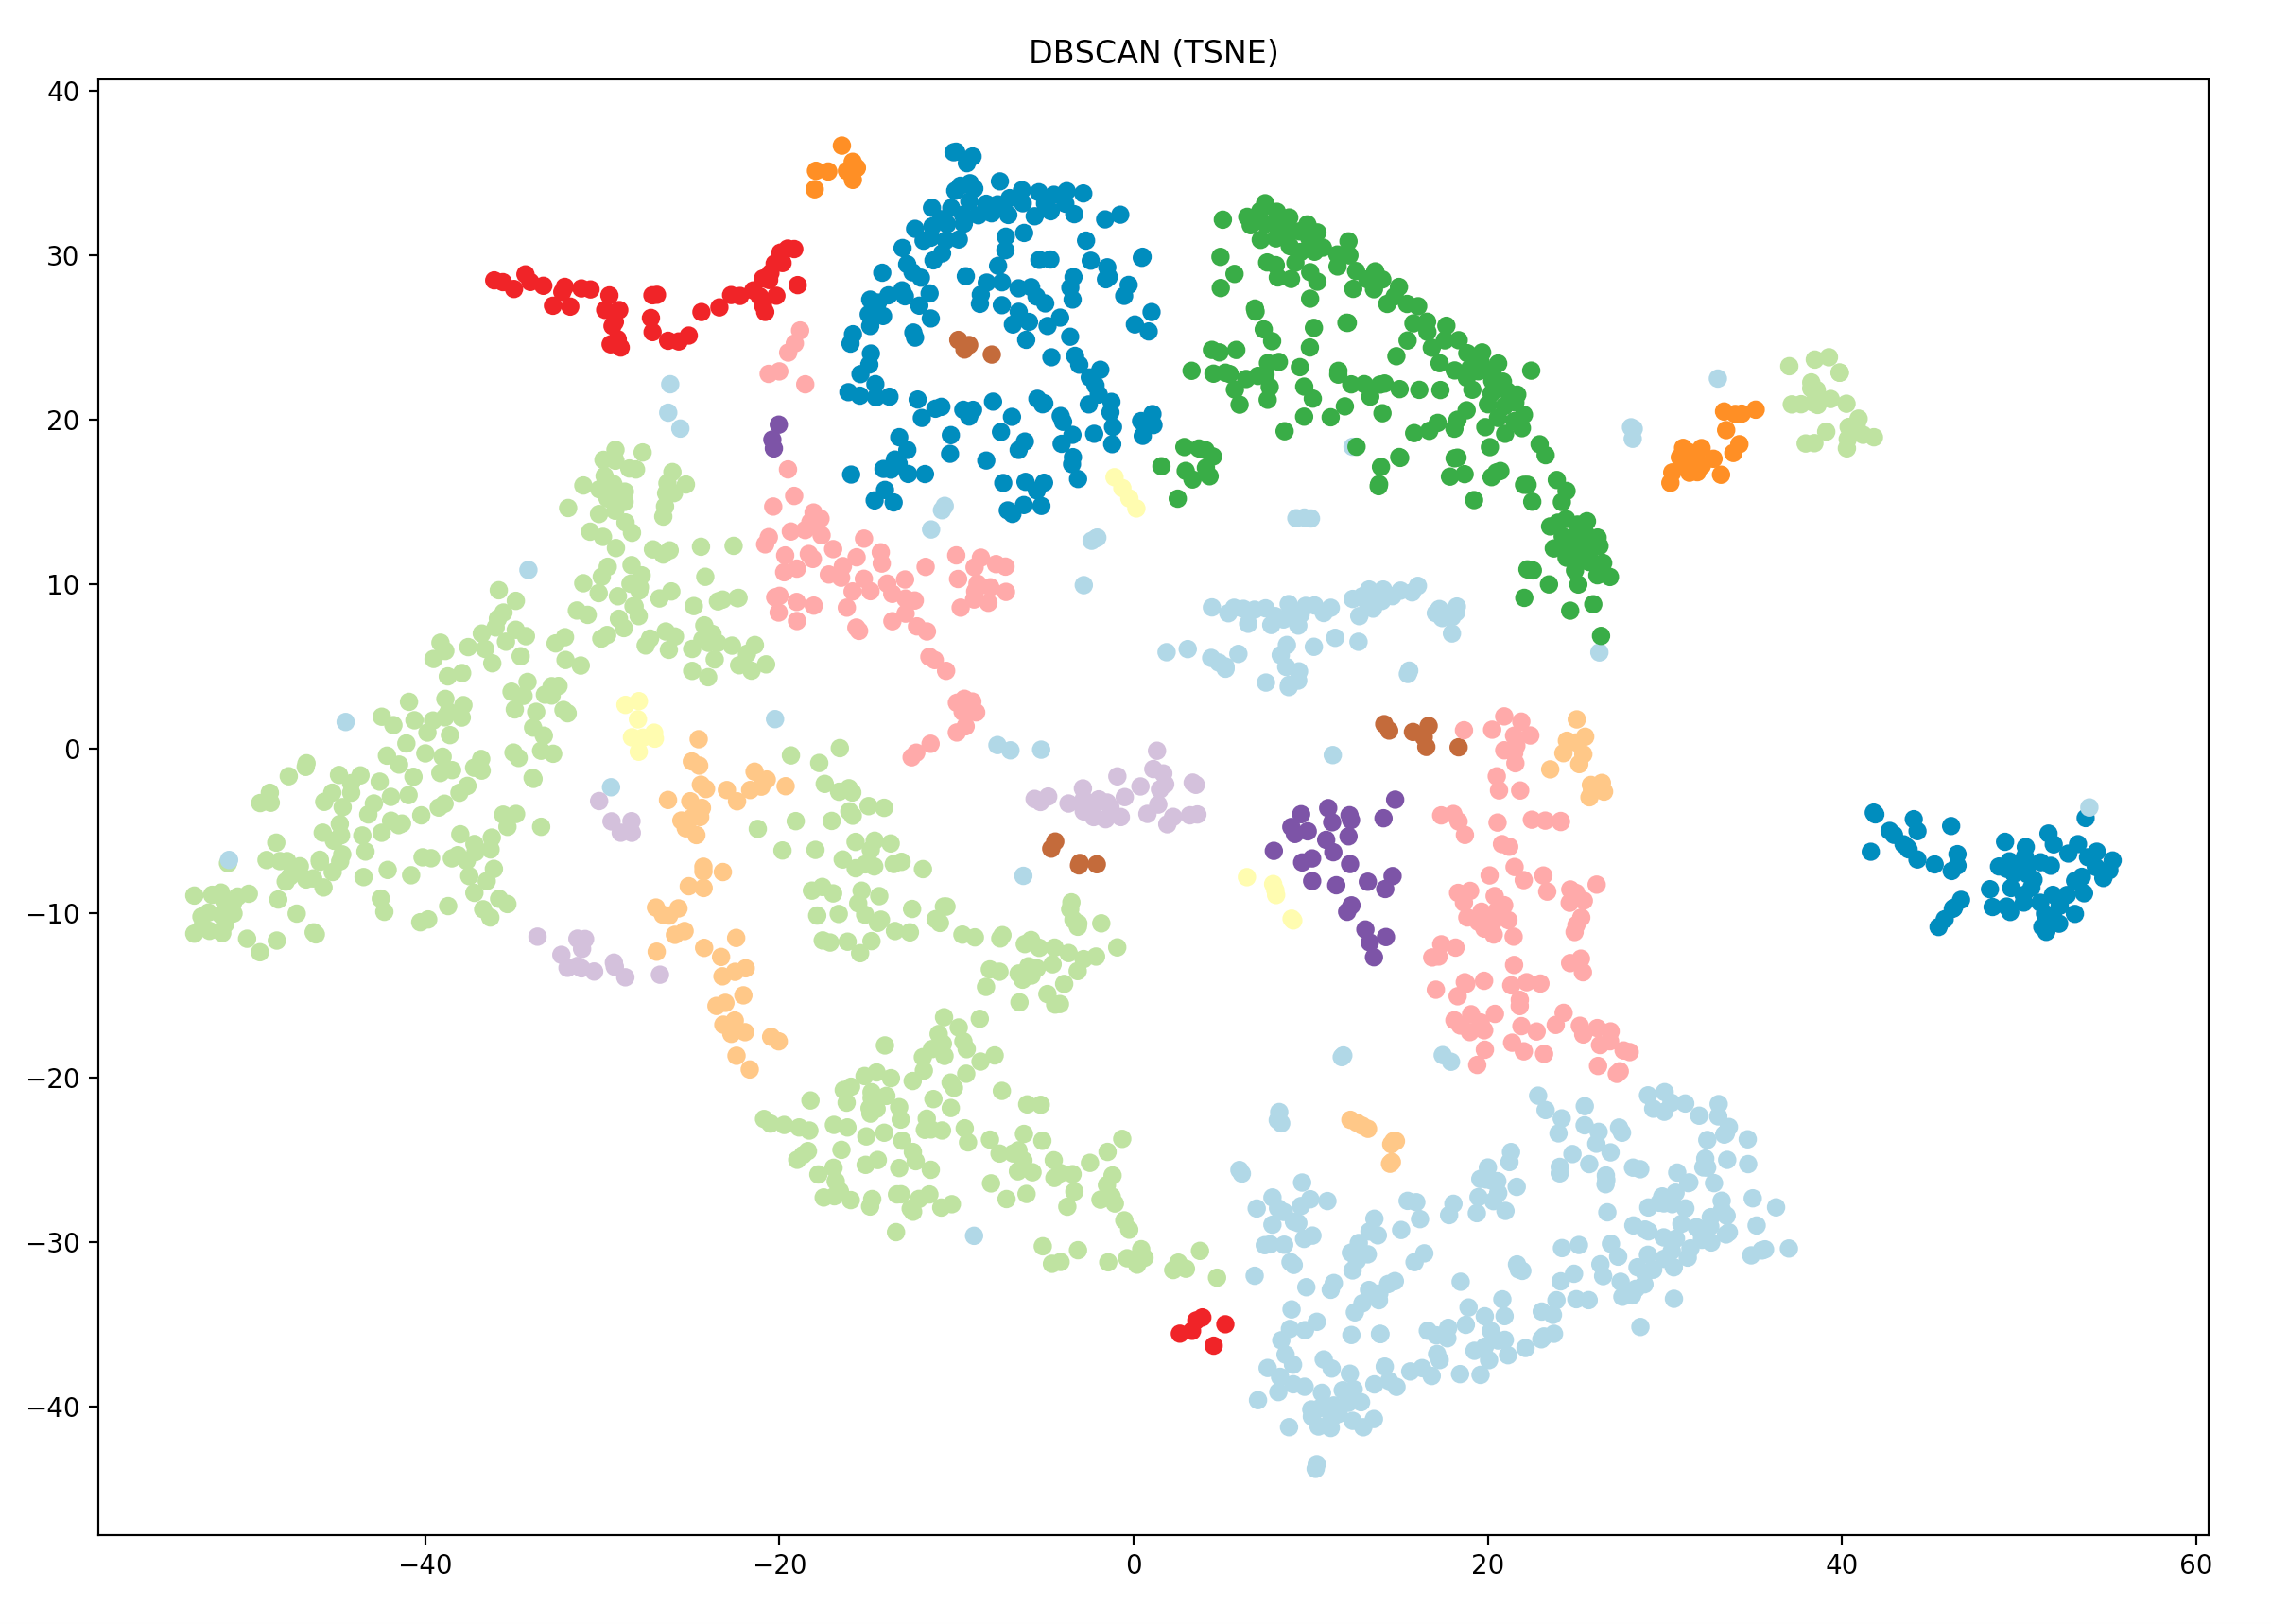
\includegraphics[width=1\textwidth]{./images/clusteringResults/1h-1-DBSCAN.png}
  \caption{1h dataset DBSCAN clustering (first column - 15 min).}
  \end{subfigure}%
  \hfill
  \begin{subfigure}{.5\textwidth}\captionsetup{width=.8\linewidth}
    \centering
    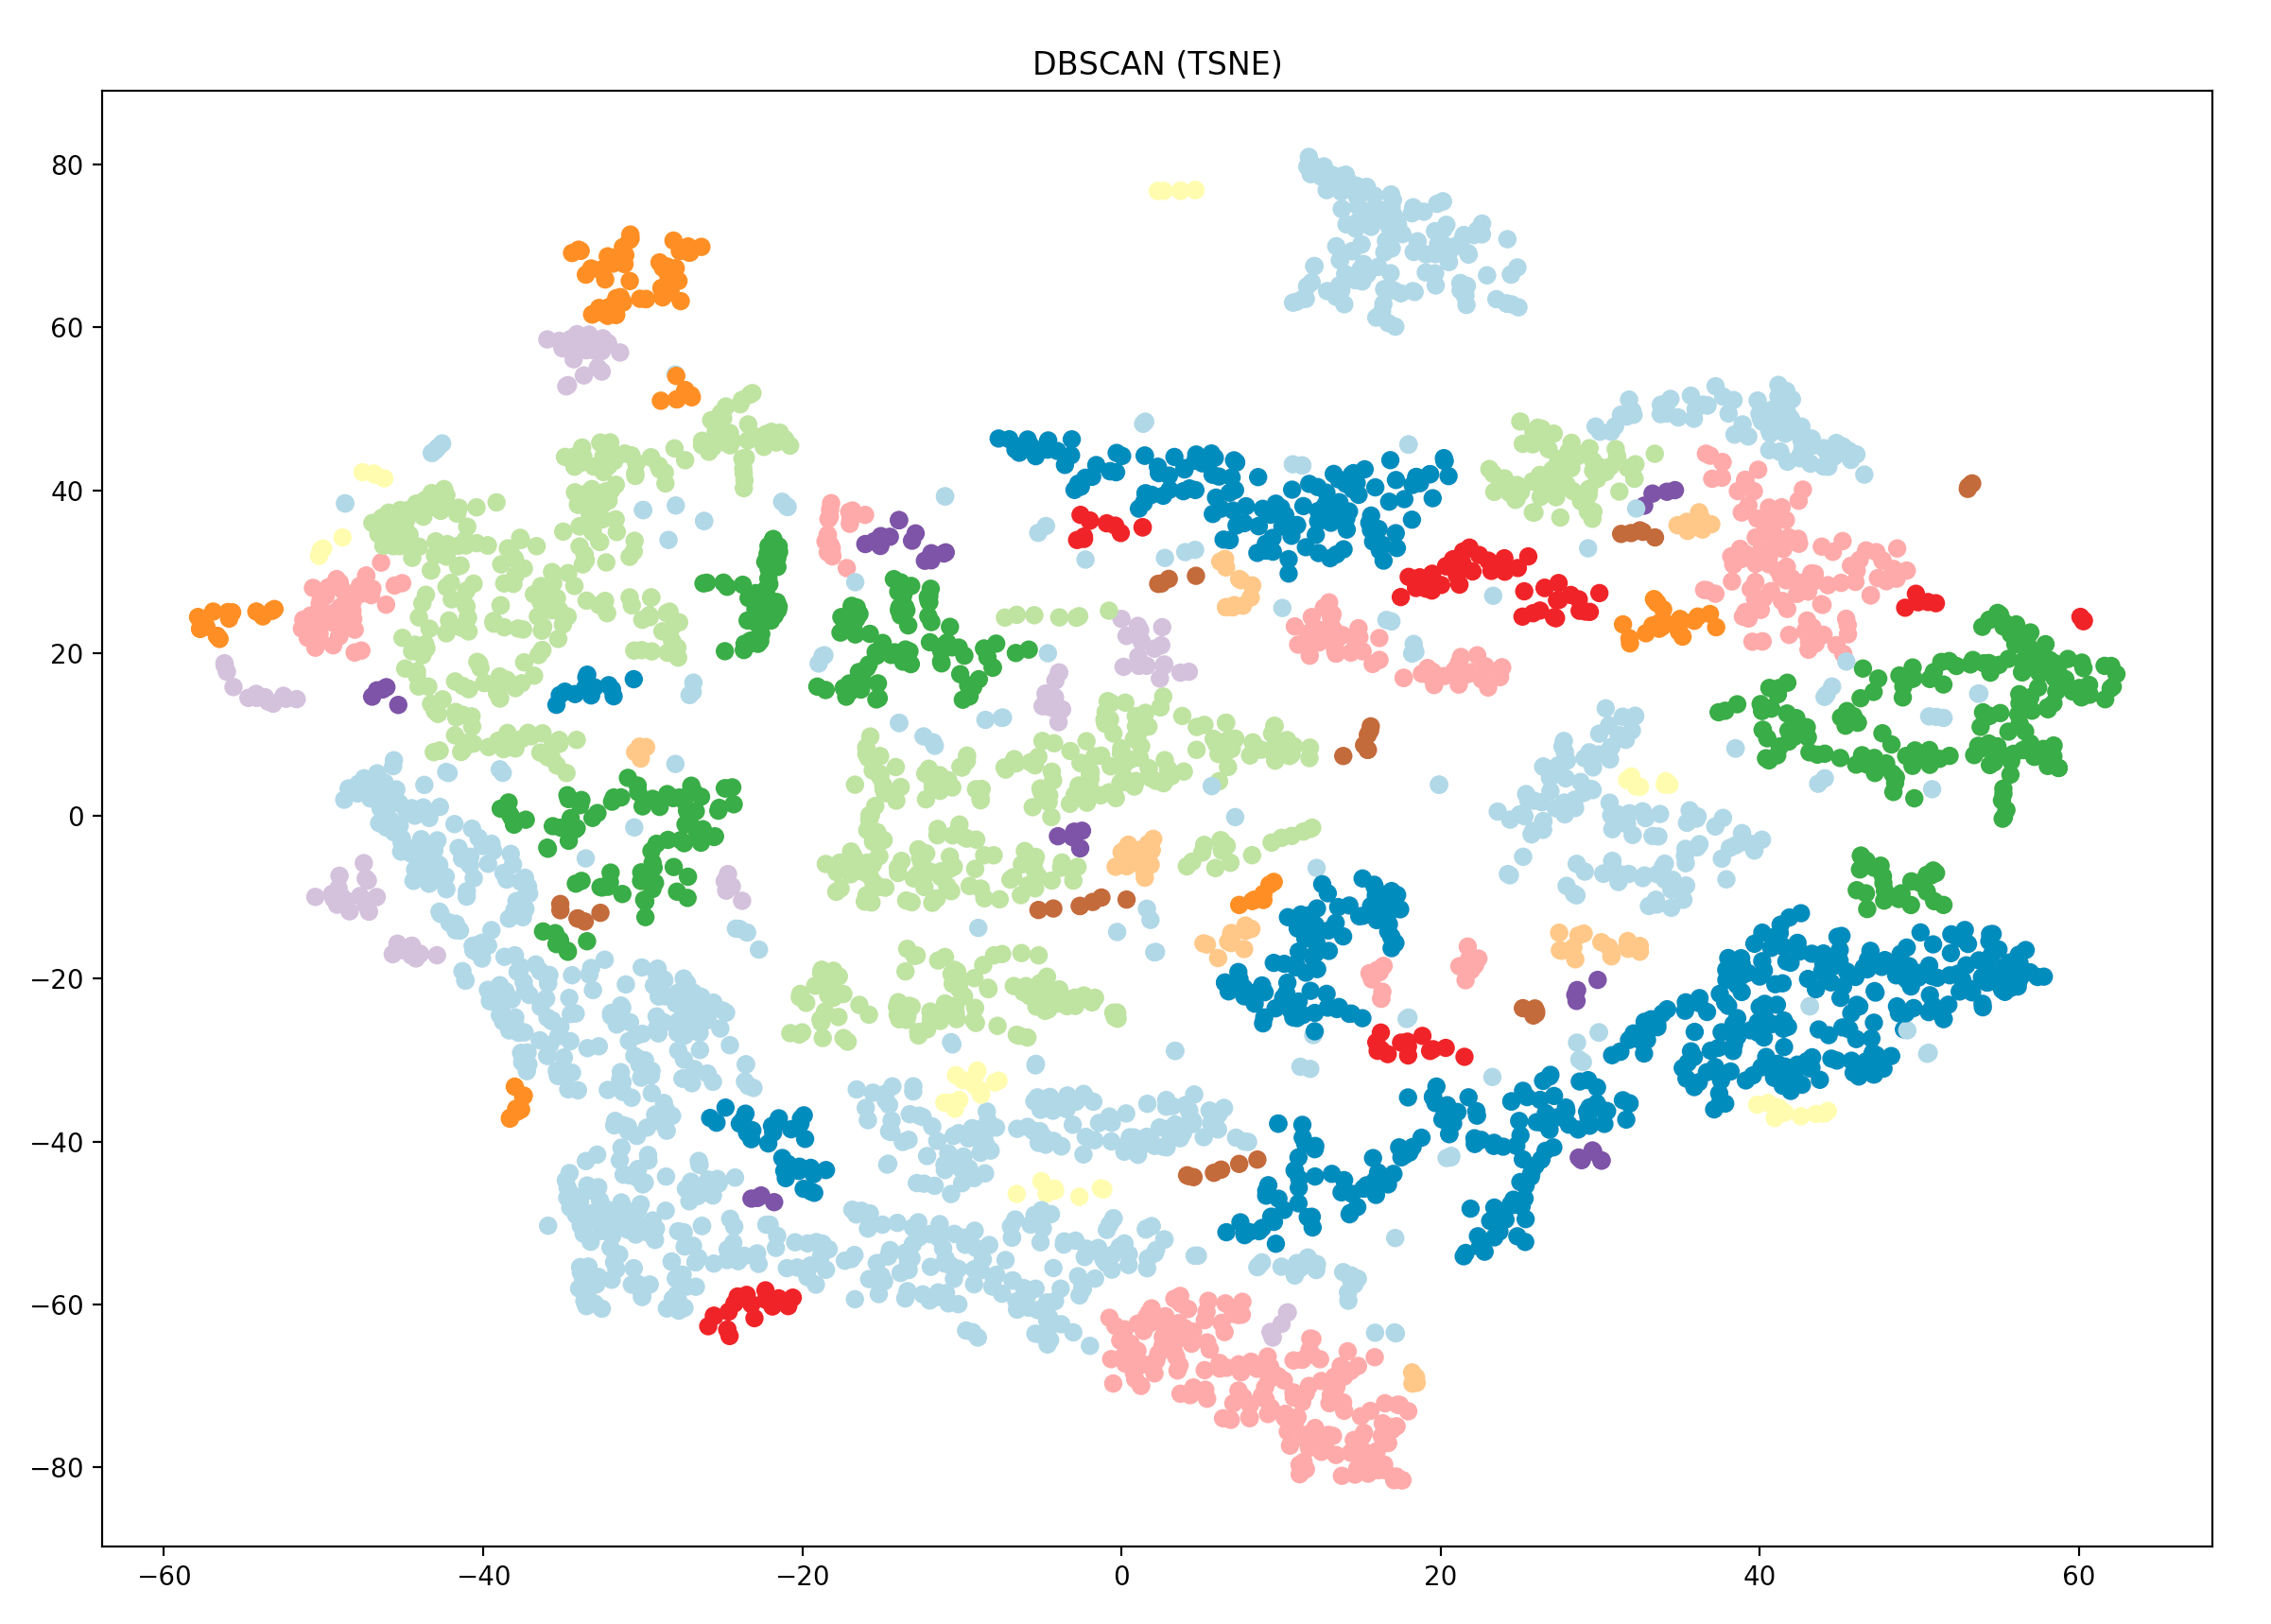
\includegraphics[width=1\textwidth]{./images/clusteringResults/3h-1-DBSCAN.png}
    \caption{3h dataset DBSCAN clustering (first column - 30 min).}
  \end{subfigure}
  \caption{}
  \label{figure:DBSCANResults}
  \end{figure}






\subsubsection{OPTICS}
The OPTICS algorithm was also implemented with its sklearn implementation\footnote{\url{https://scikit-learn.org/stable/modules/generated/sklearn.cluster.OPTICS.html}}. As stated in section \ref{section:OPTICS}, the OPTICS algorithm creates a reachability plot for the data points. Initially, the clusters were extracted using the clustering method "xi". This is the automatic cluster extraction method, as explained in section \ref{section:OPTICS} and introduced in \textcite{OPTICS}[57]. The visual results of these clusterings appeared to contain many points that were not assigned to clusters, as can be seen in figure \ref{figure:OPTICSXiResults}. Moreover, the corresponding reachability plots showed many points that weren't assigned to a cluster (no colour). This resulted in the DBSCAN method being used to cluster the OPTICS results. The Eps parameter was set to 2, as determined before for the DBSCAN clustering algorithm. The resulting clusters are depicted in figure \ref{figure:OPTICSResults}. The corresponding reachability plots are illustrated in figure \ref{figure:OPTICSResultsReachabilityPlot}.


\begin{figure}[H]
  \centering
  \begin{subfigure}{.5\textwidth}\captionsetup{width=.8\linewidth}
    \centering
    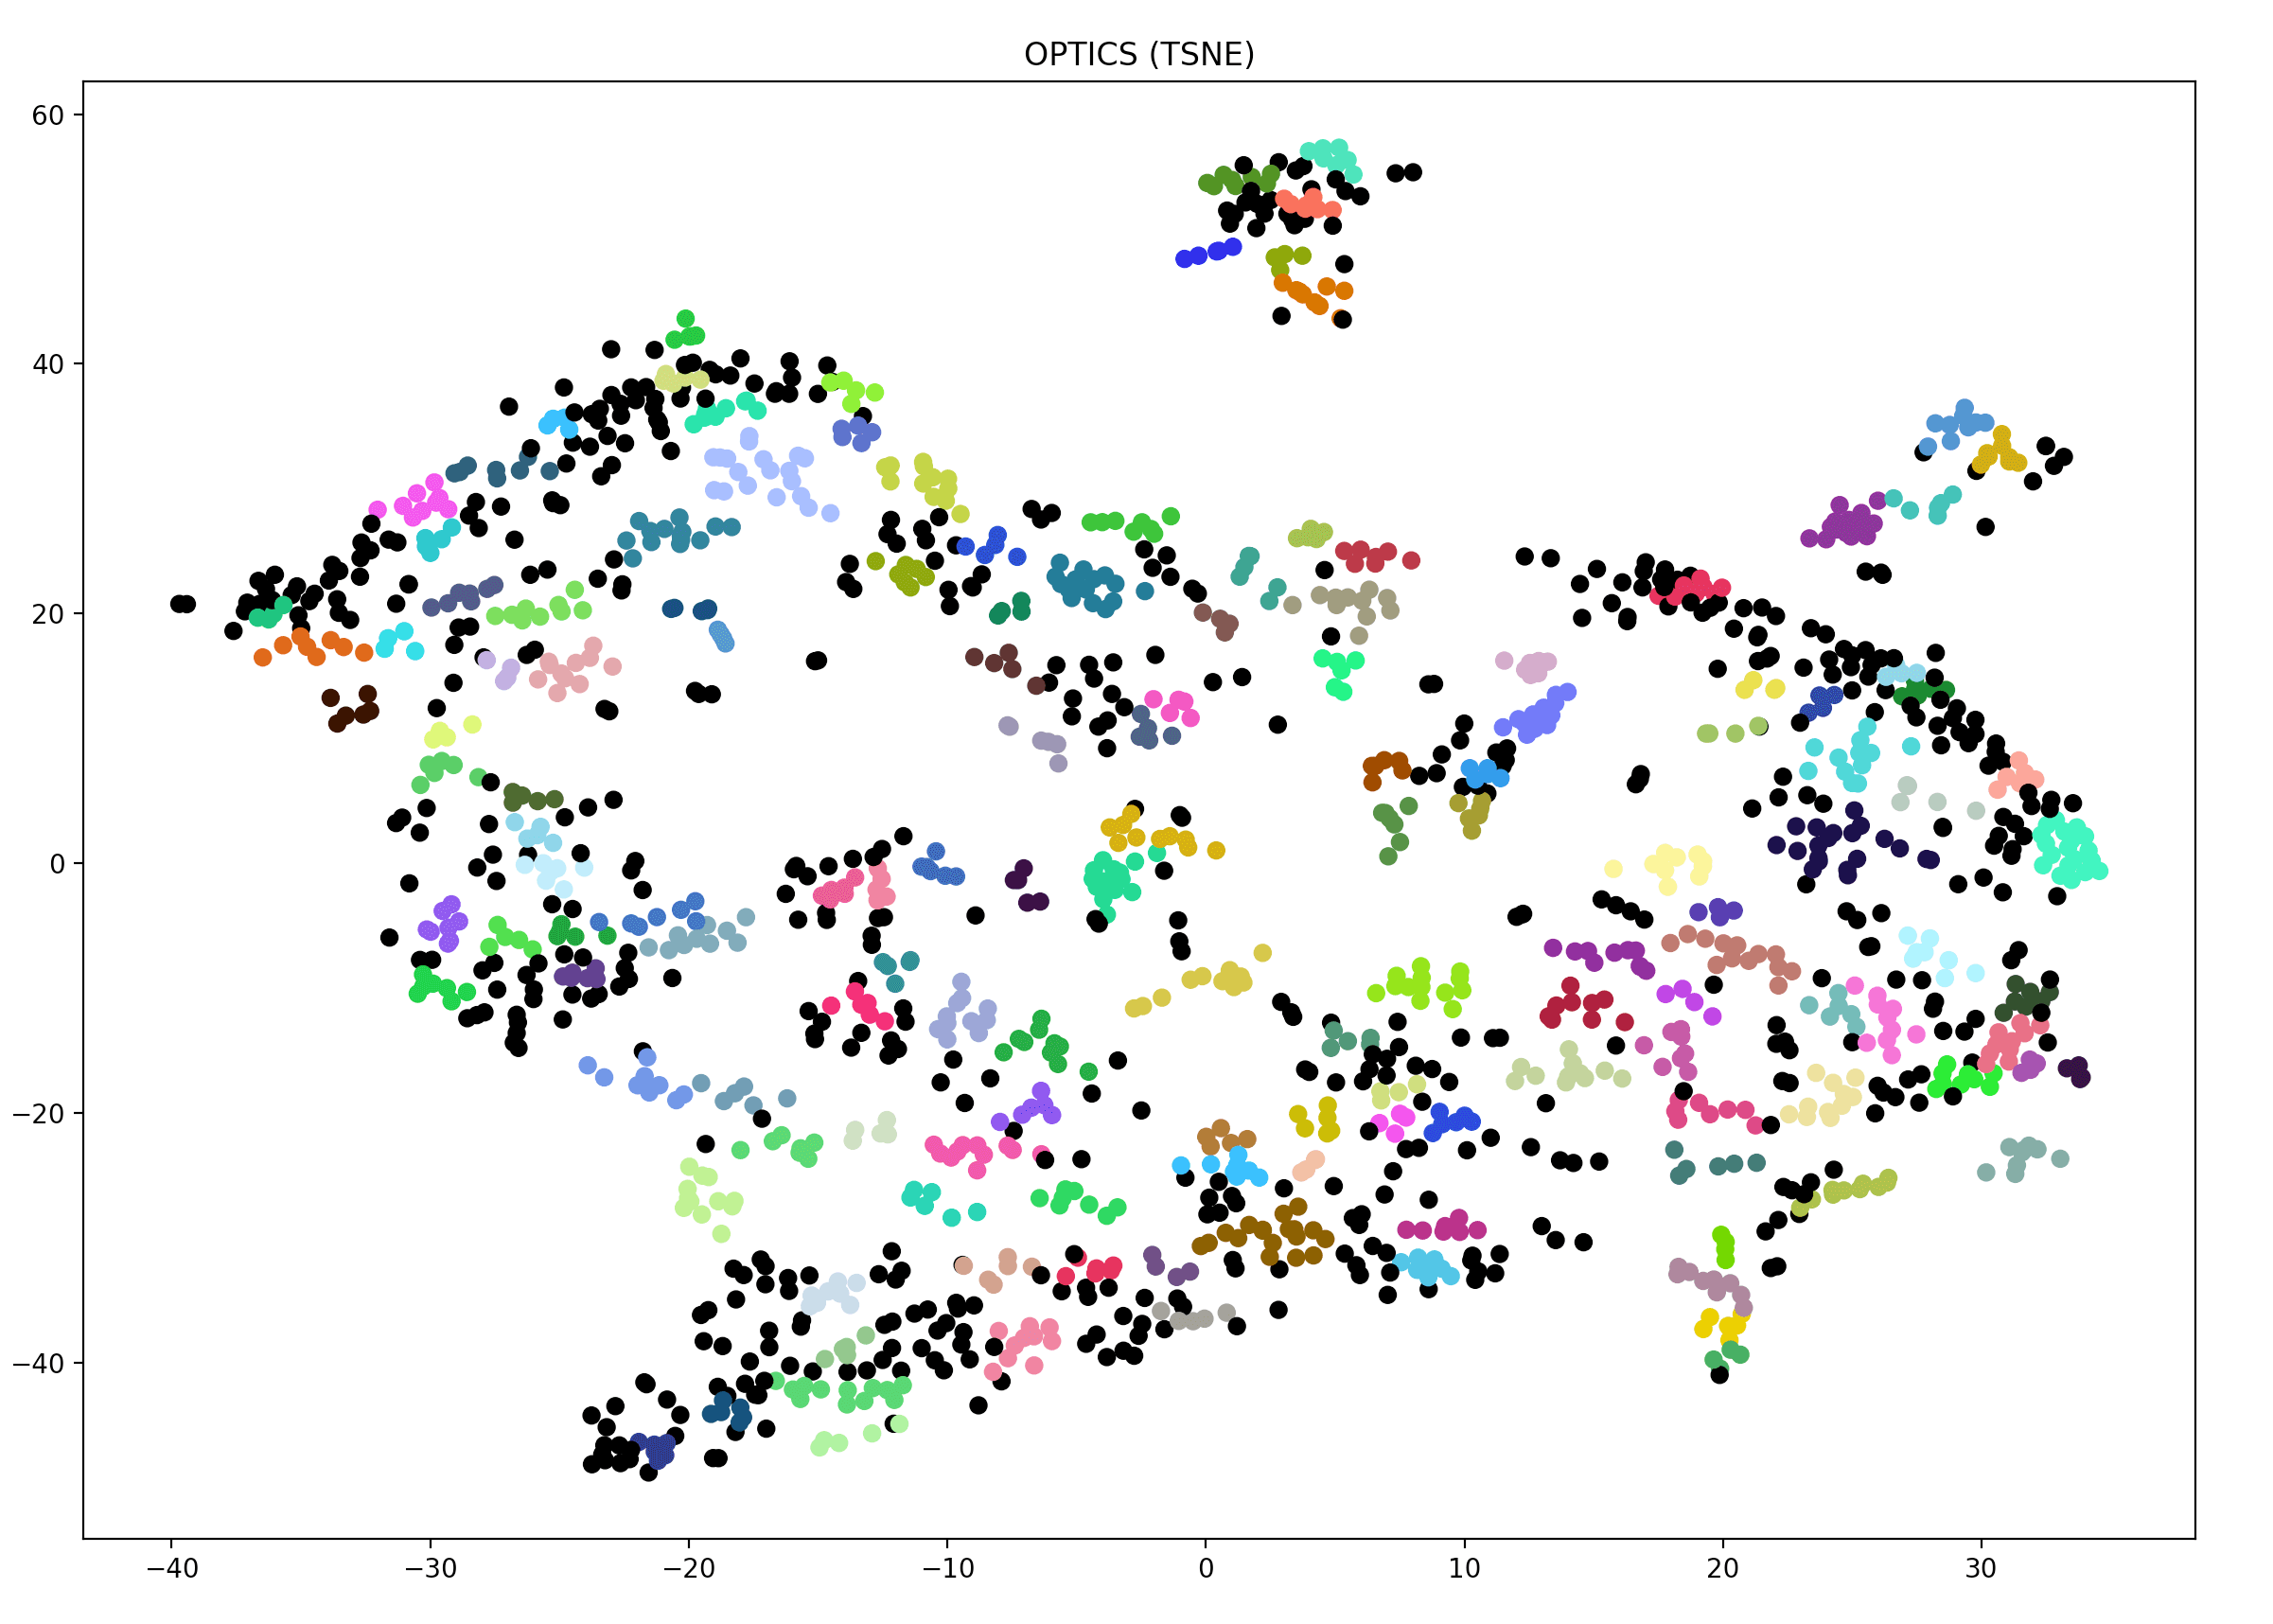
\includegraphics[width=1\textwidth]{./images/OPTICS/1h-1-OPTICS-xi.png}
  \caption{1h dataset OPTICS clustering (first column - 30 min), using OPTICS automatic cluster extraction (xi).}
  \end{subfigure}%
  \hfill
  \begin{subfigure}{.5\textwidth}\captionsetup{width=.8\linewidth}
    \centering
    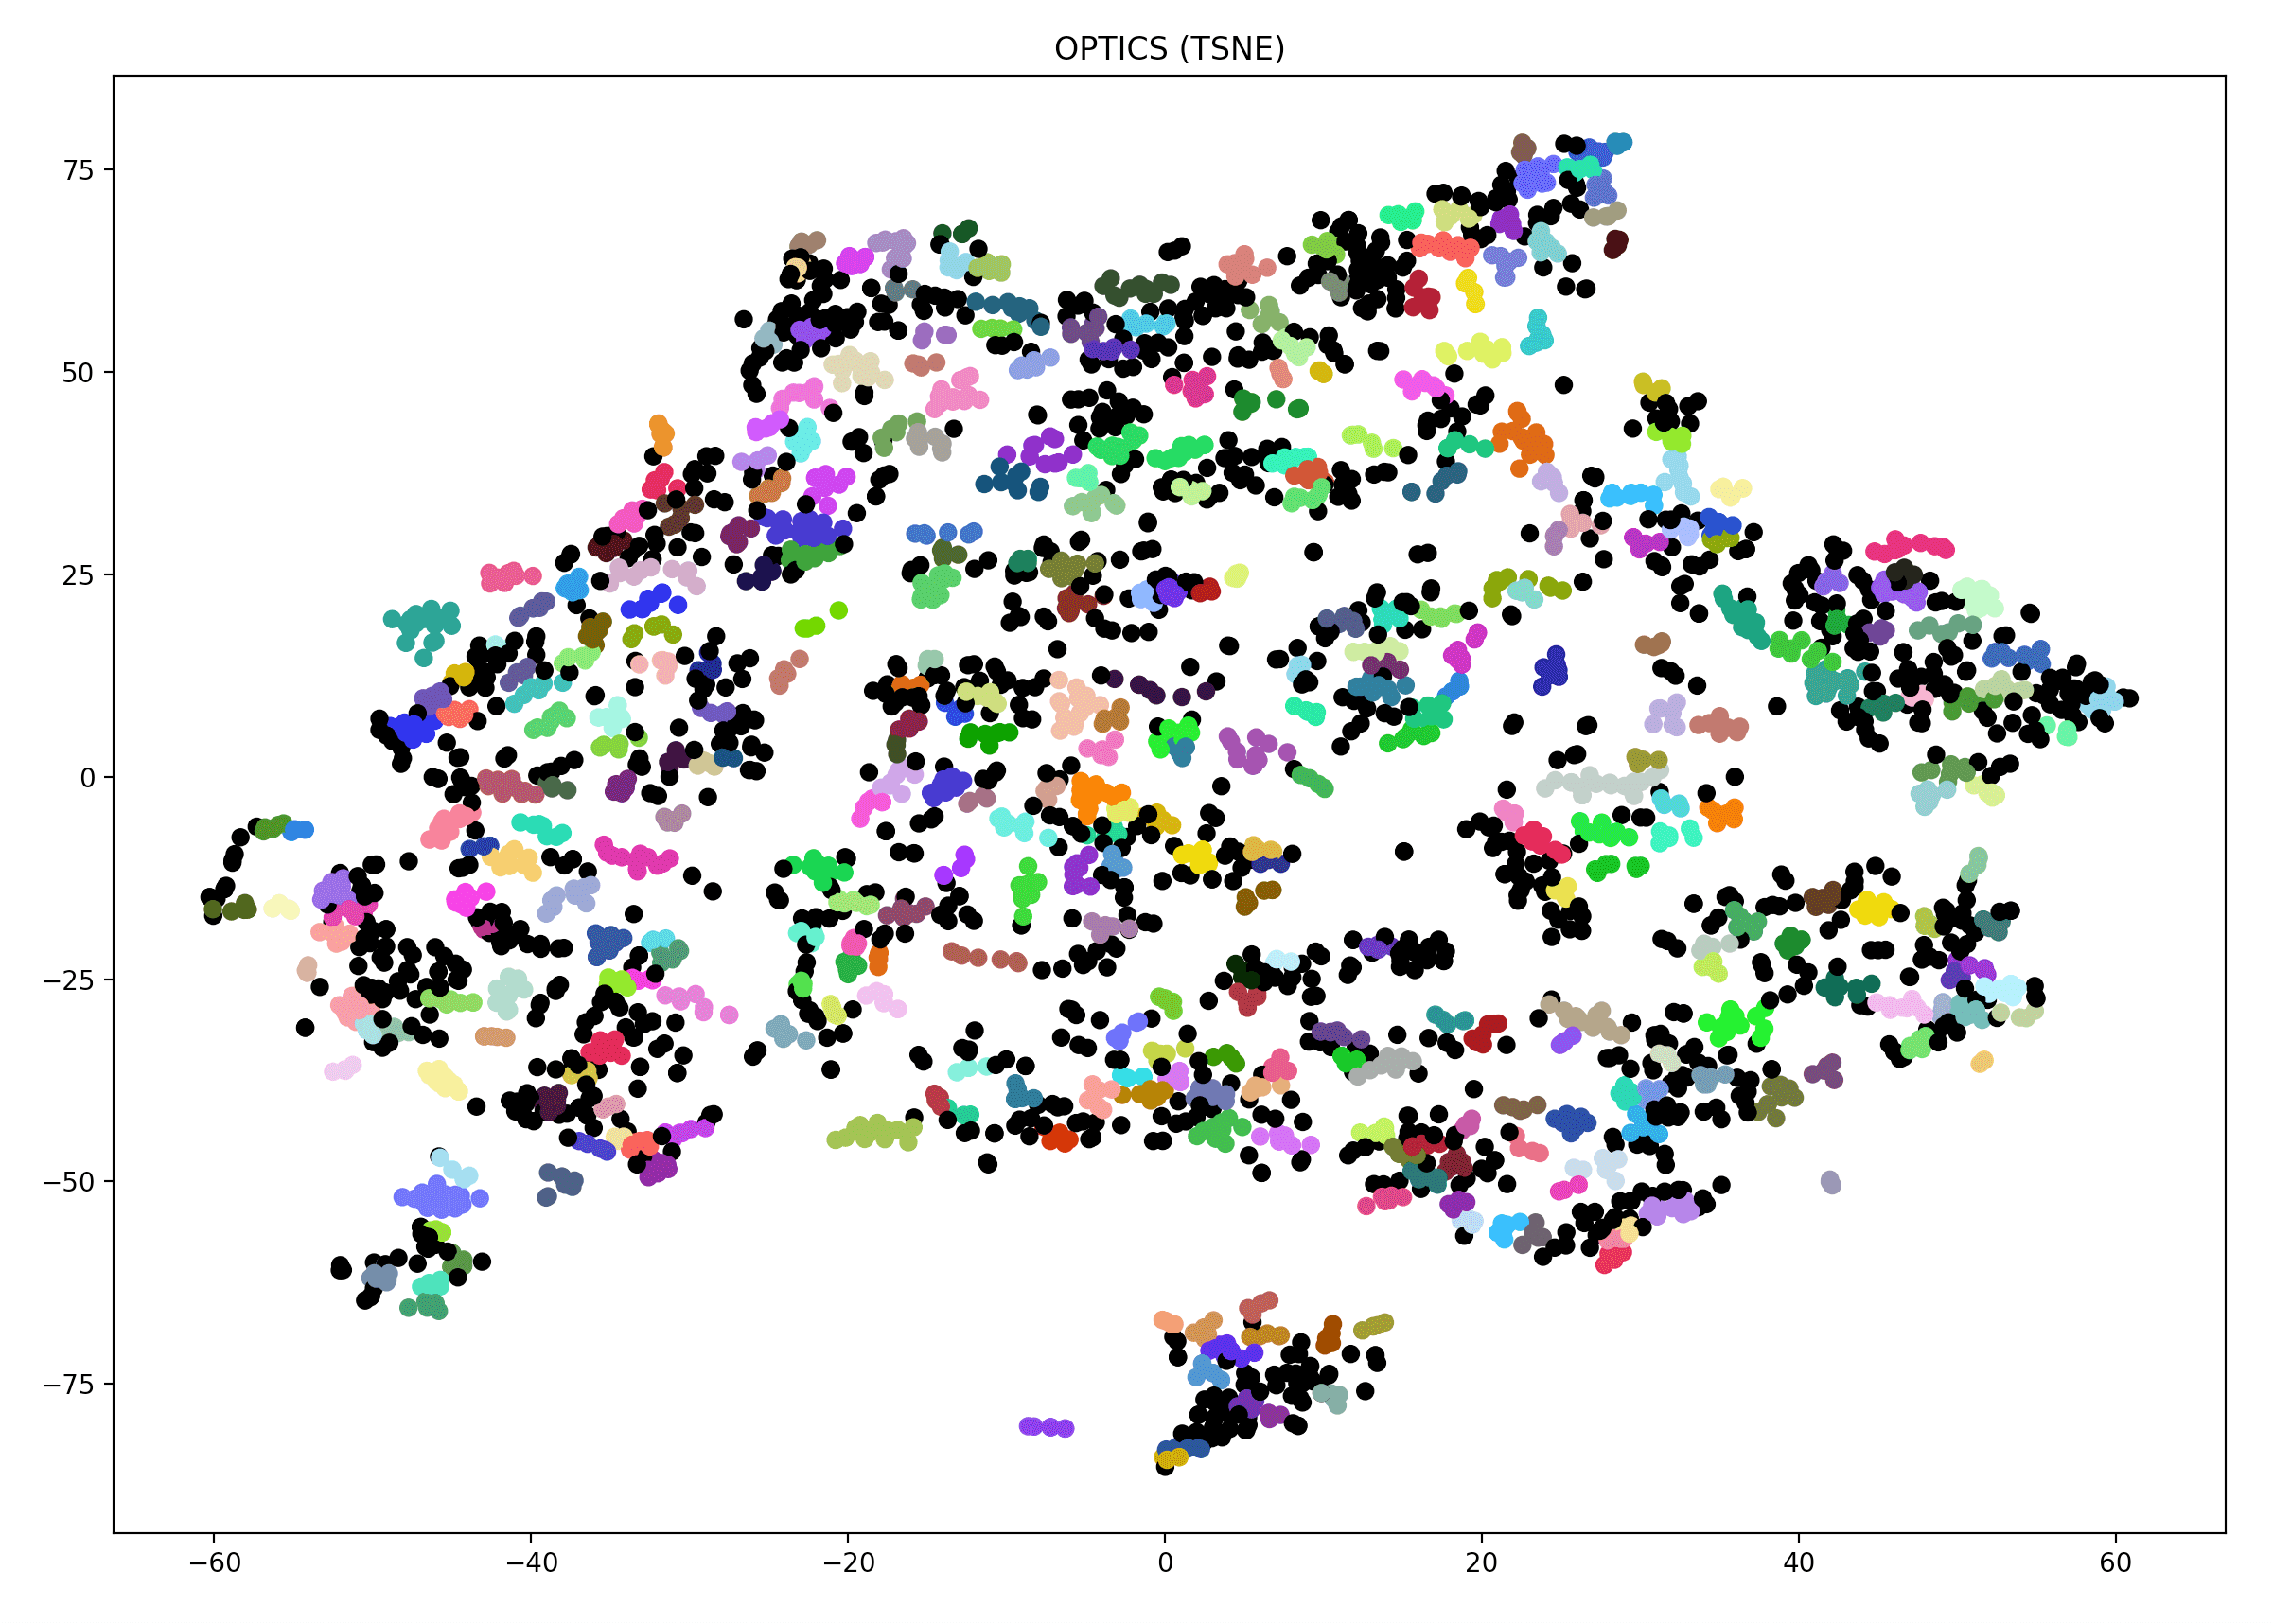
\includegraphics[width=1\textwidth]{./images/OPTICS/3h-1-OPTICS-xi.png}
    \caption{3h dataset OPTICS clustering (first column - 30 min), using OPTICS automatic cluster extraction (xi).}
  \end{subfigure}
  \caption{}
  \label{figure:OPTICSXiResults}
  \end{figure}

  \begin{figure}[H]
    \centering
    \begin{subfigure}{.5\textwidth}\captionsetup{width=.8\linewidth}
      \centering
      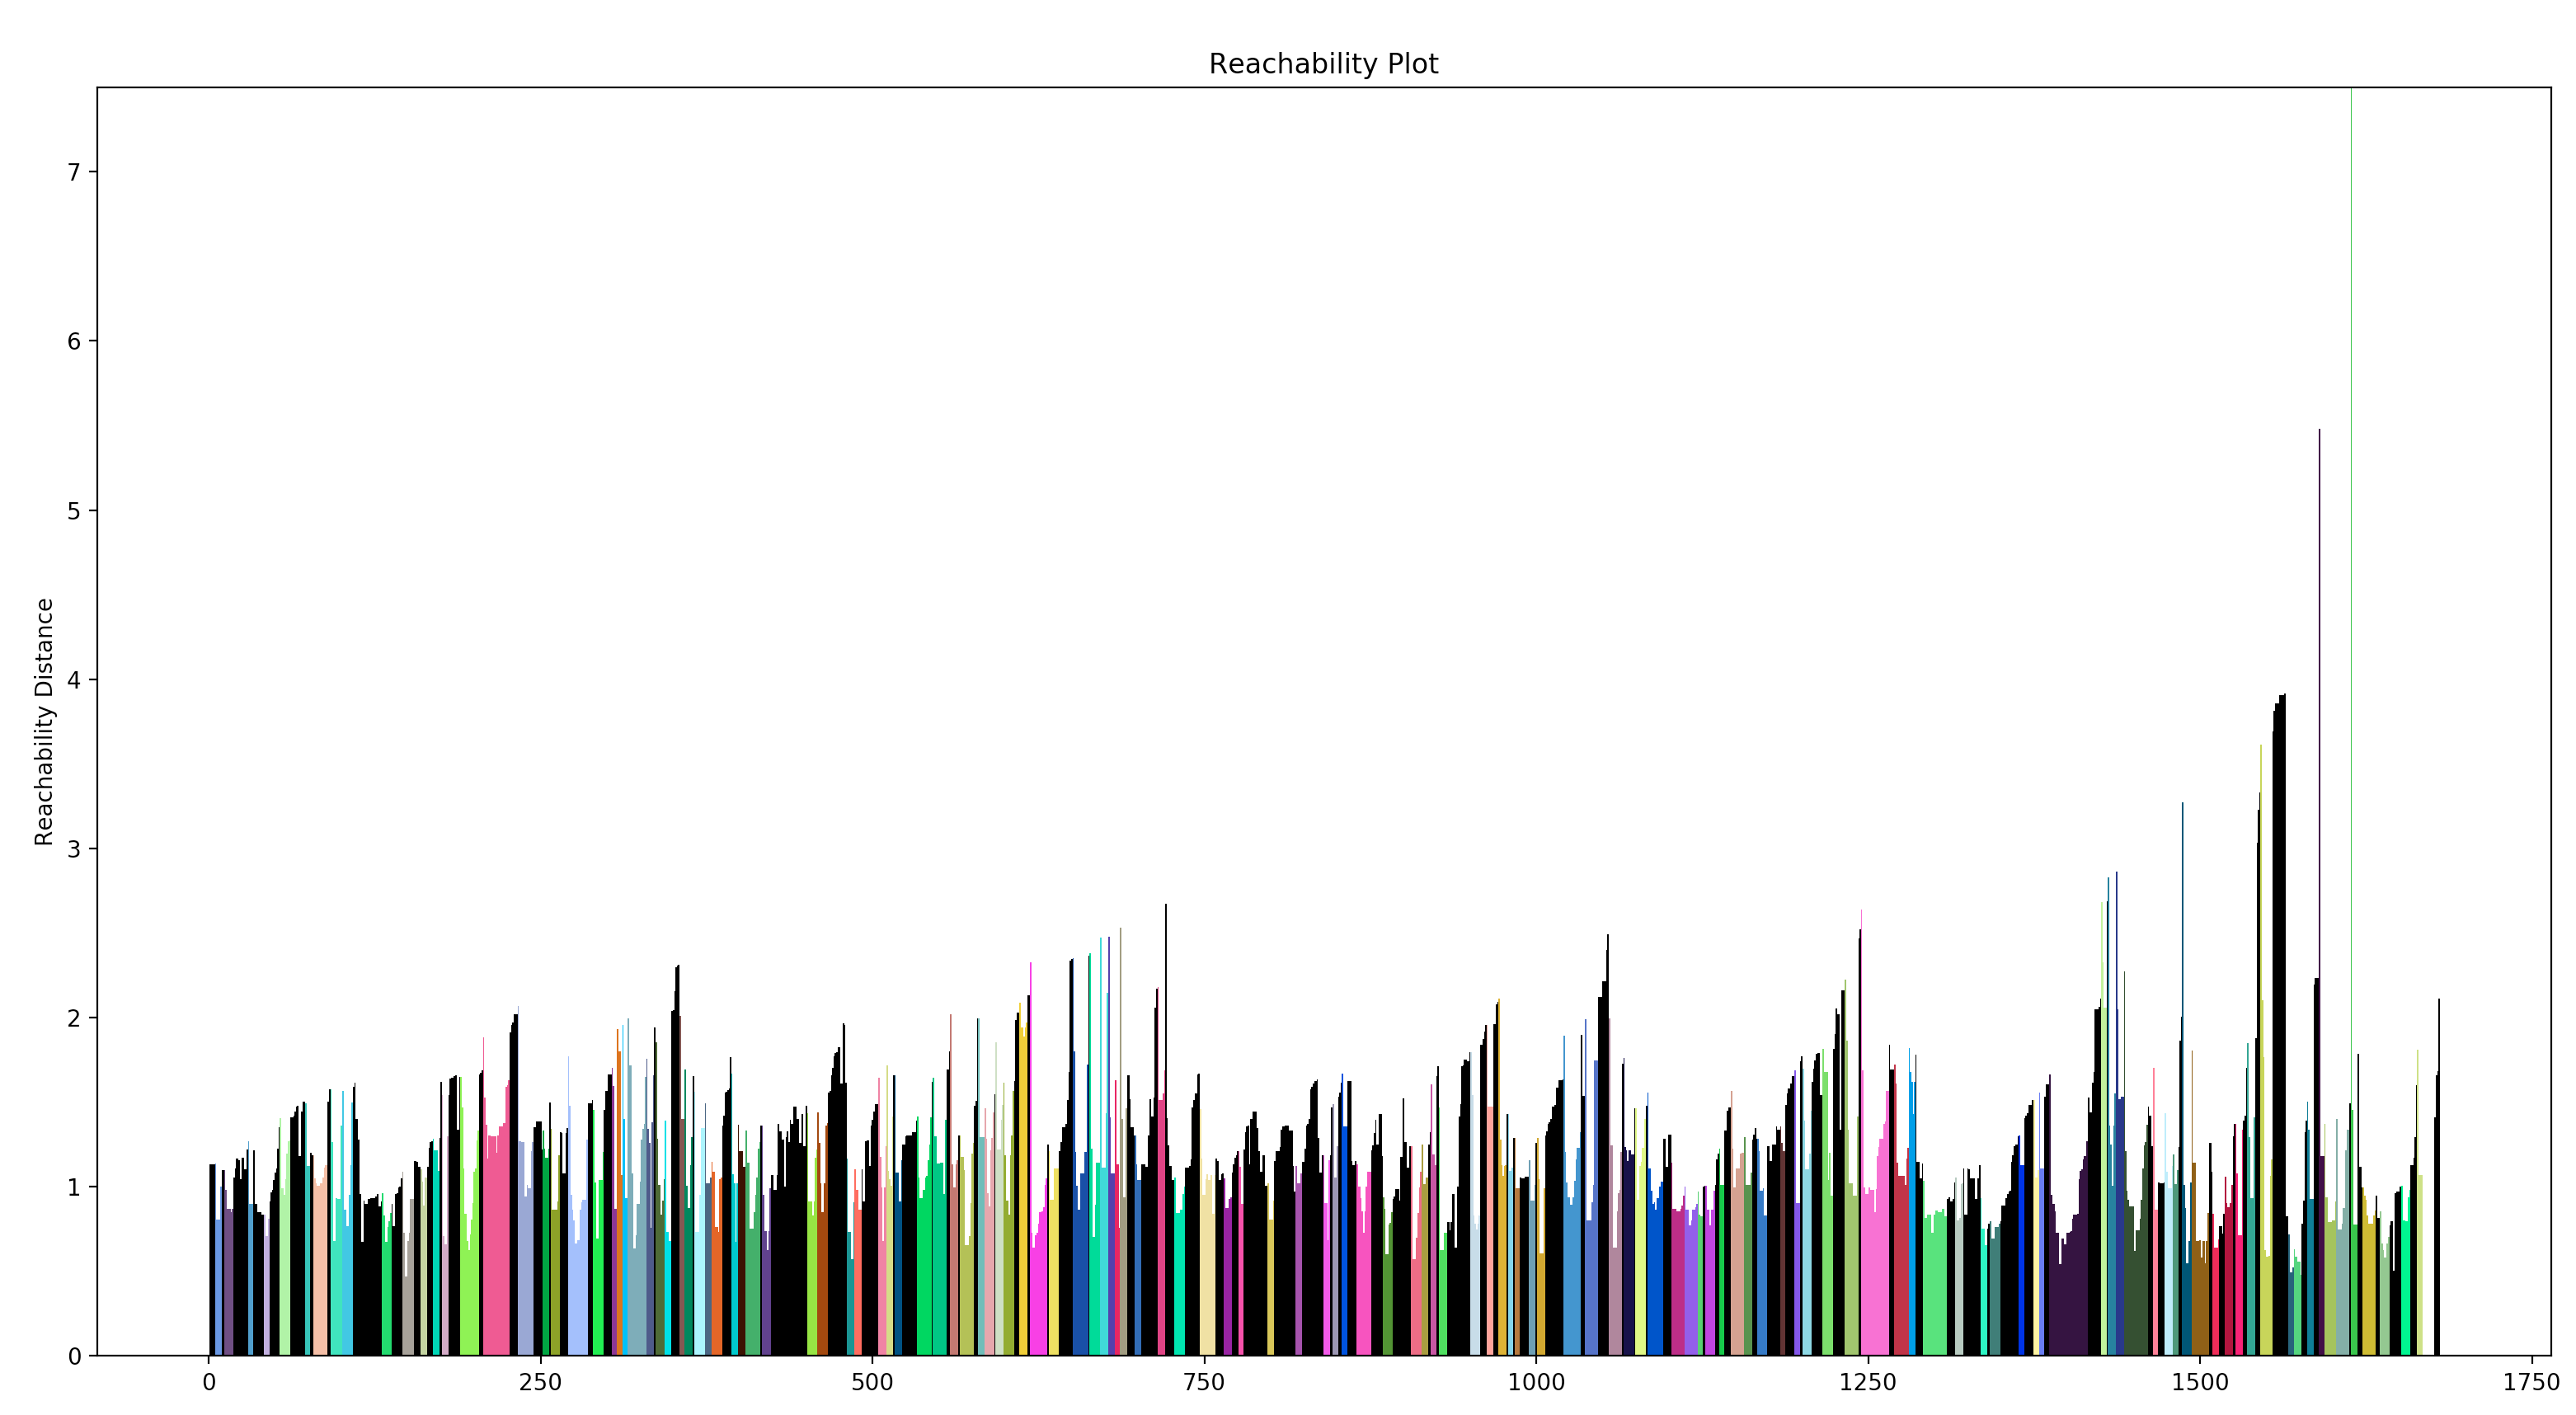
\includegraphics[width=1\textwidth]{./images/OPTICS/1h-1-reachabilityPlot-xi.png}
    \caption{1h dataset OPTICS reachability plot (first column - 15 min), using OPTICS automatic cluster extraction (xi).}
    \end{subfigure}%
    \begin{subfigure}{.5\textwidth}\captionsetup{width=.8\linewidth}
      \centering
      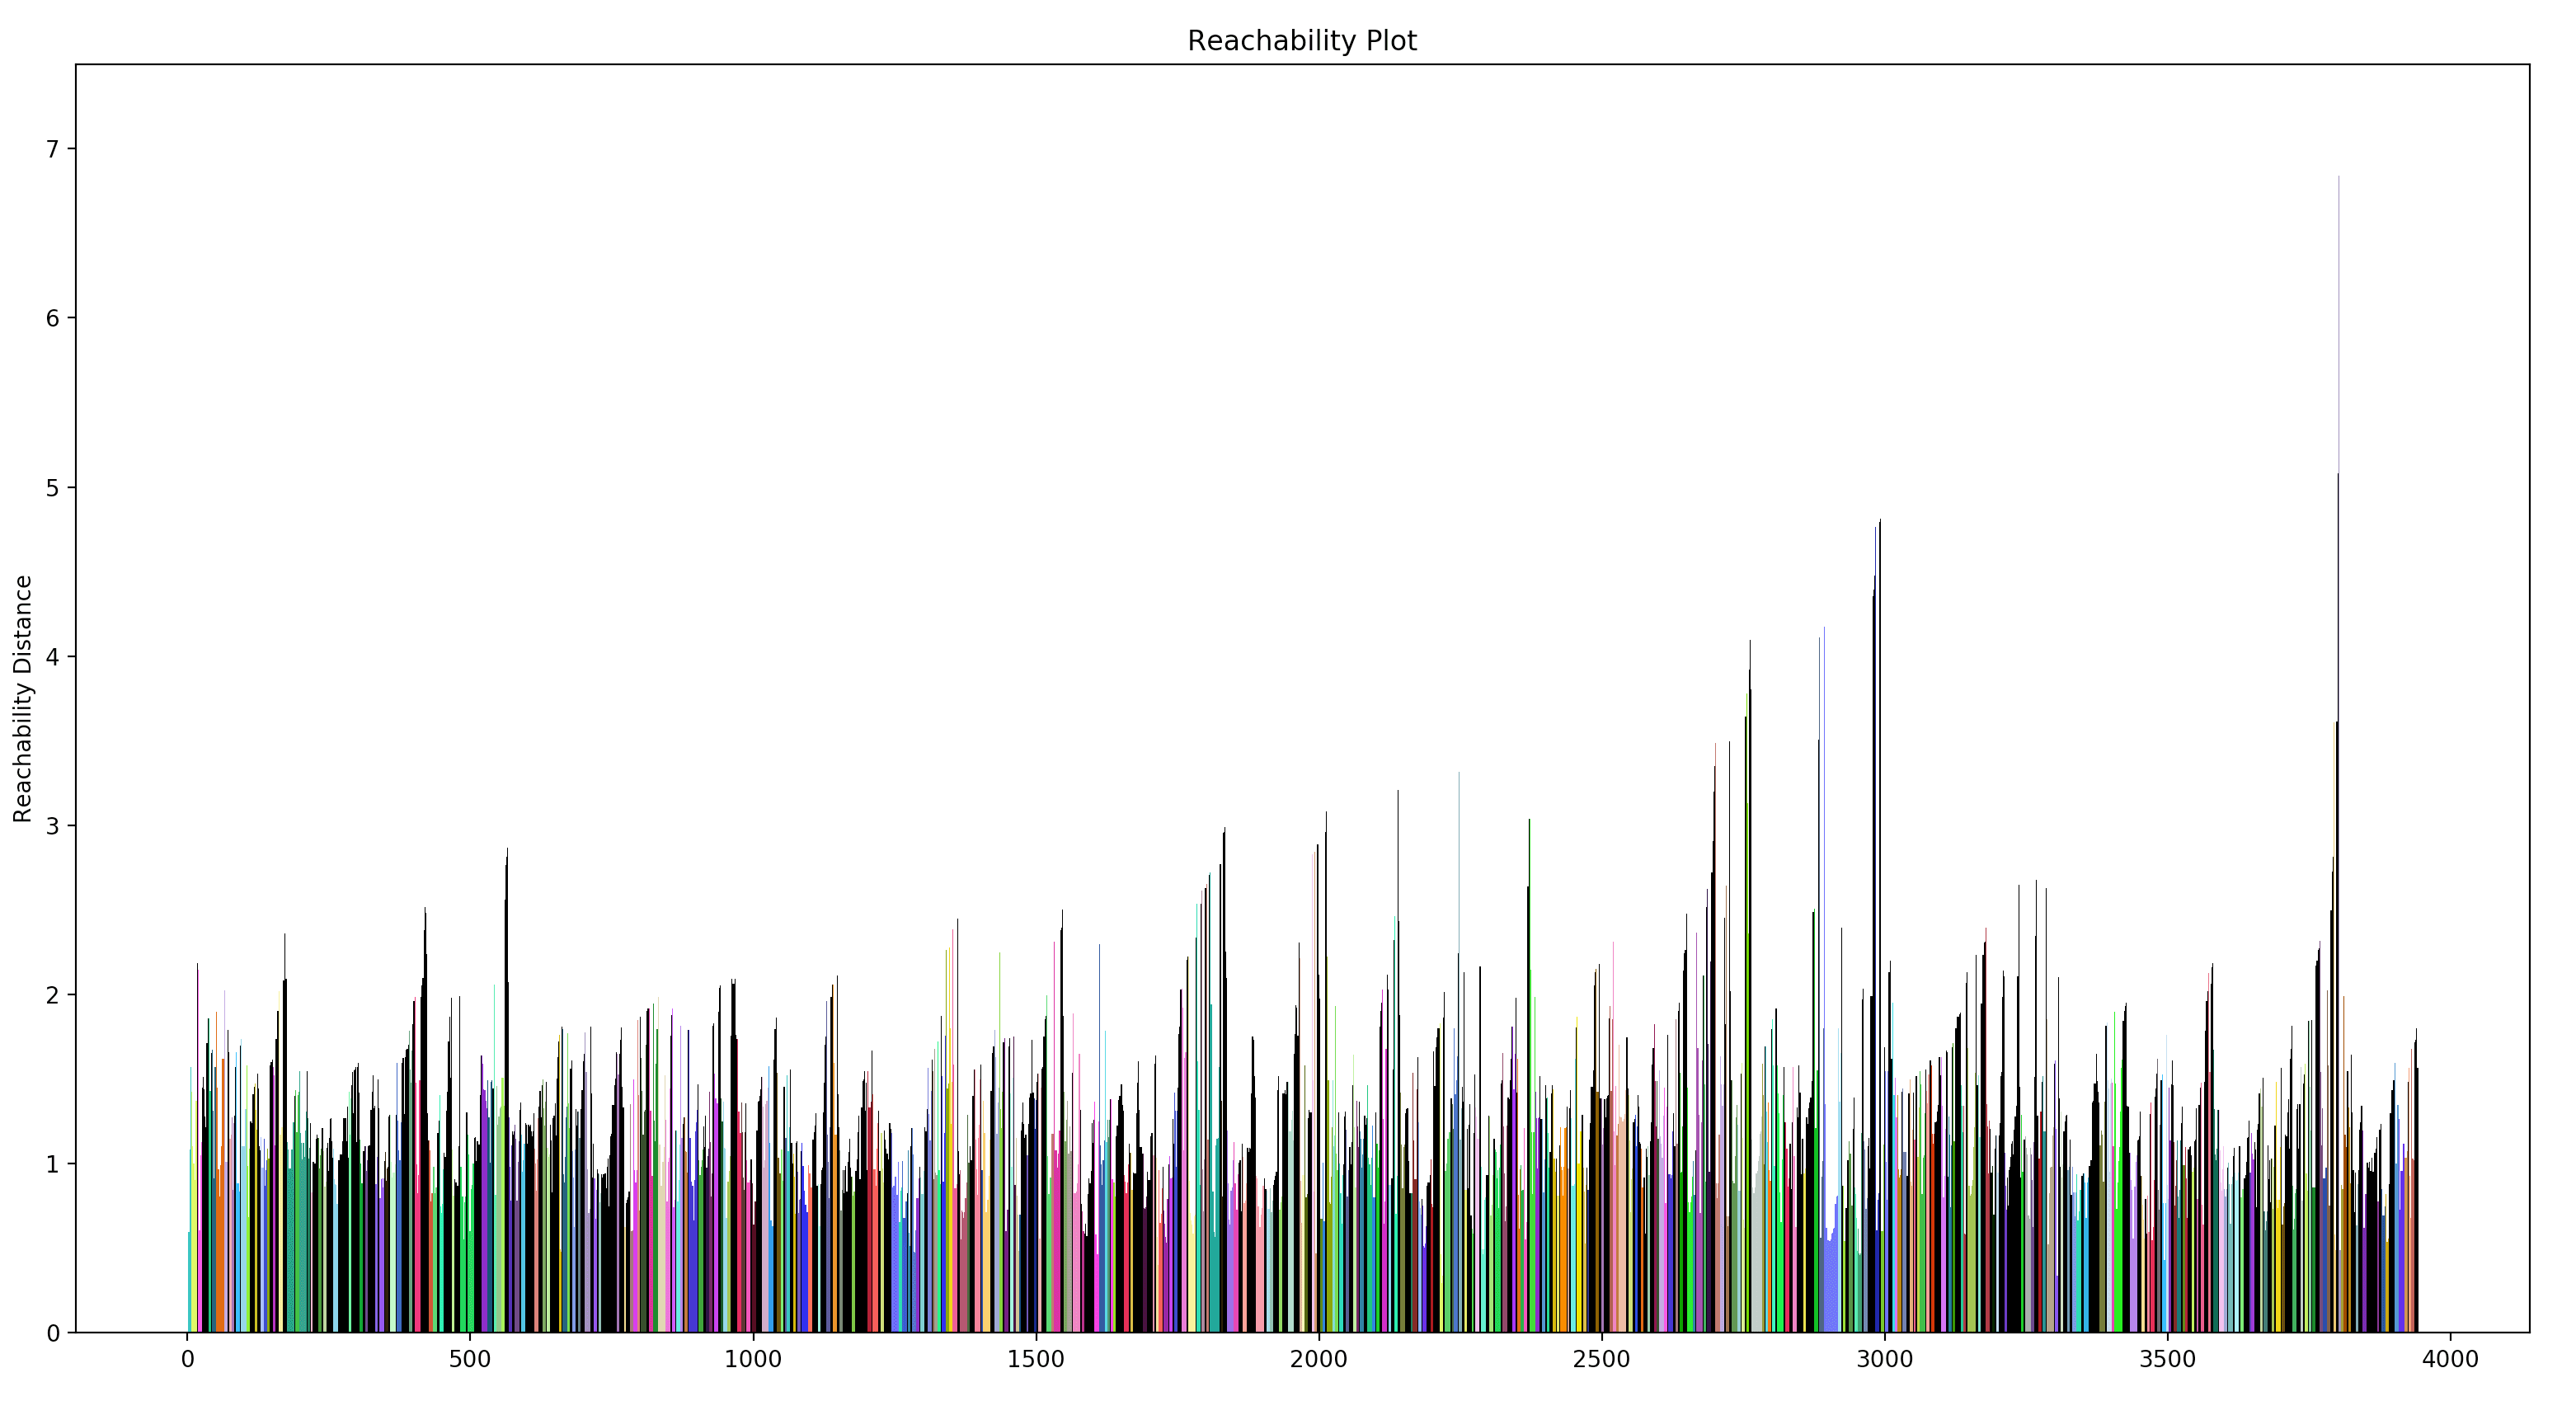
\includegraphics[width=1\textwidth]{./images/OPTICS/3h-1-reachabilityPlot-xi.png}
      \caption{3h dataset OPTICS reachability plot (first column - 30 min), using OPTICS automatic cluster extraction (xi).}
    \end{subfigure}
    \caption{}
    \label{figure:OPTICSResultsReachabilityPlot}
    \end{figure}

\begin{figure}[H]
  \centering
  \begin{subfigure}{.5\textwidth}\captionsetup{width=.8\linewidth}
    \centering
    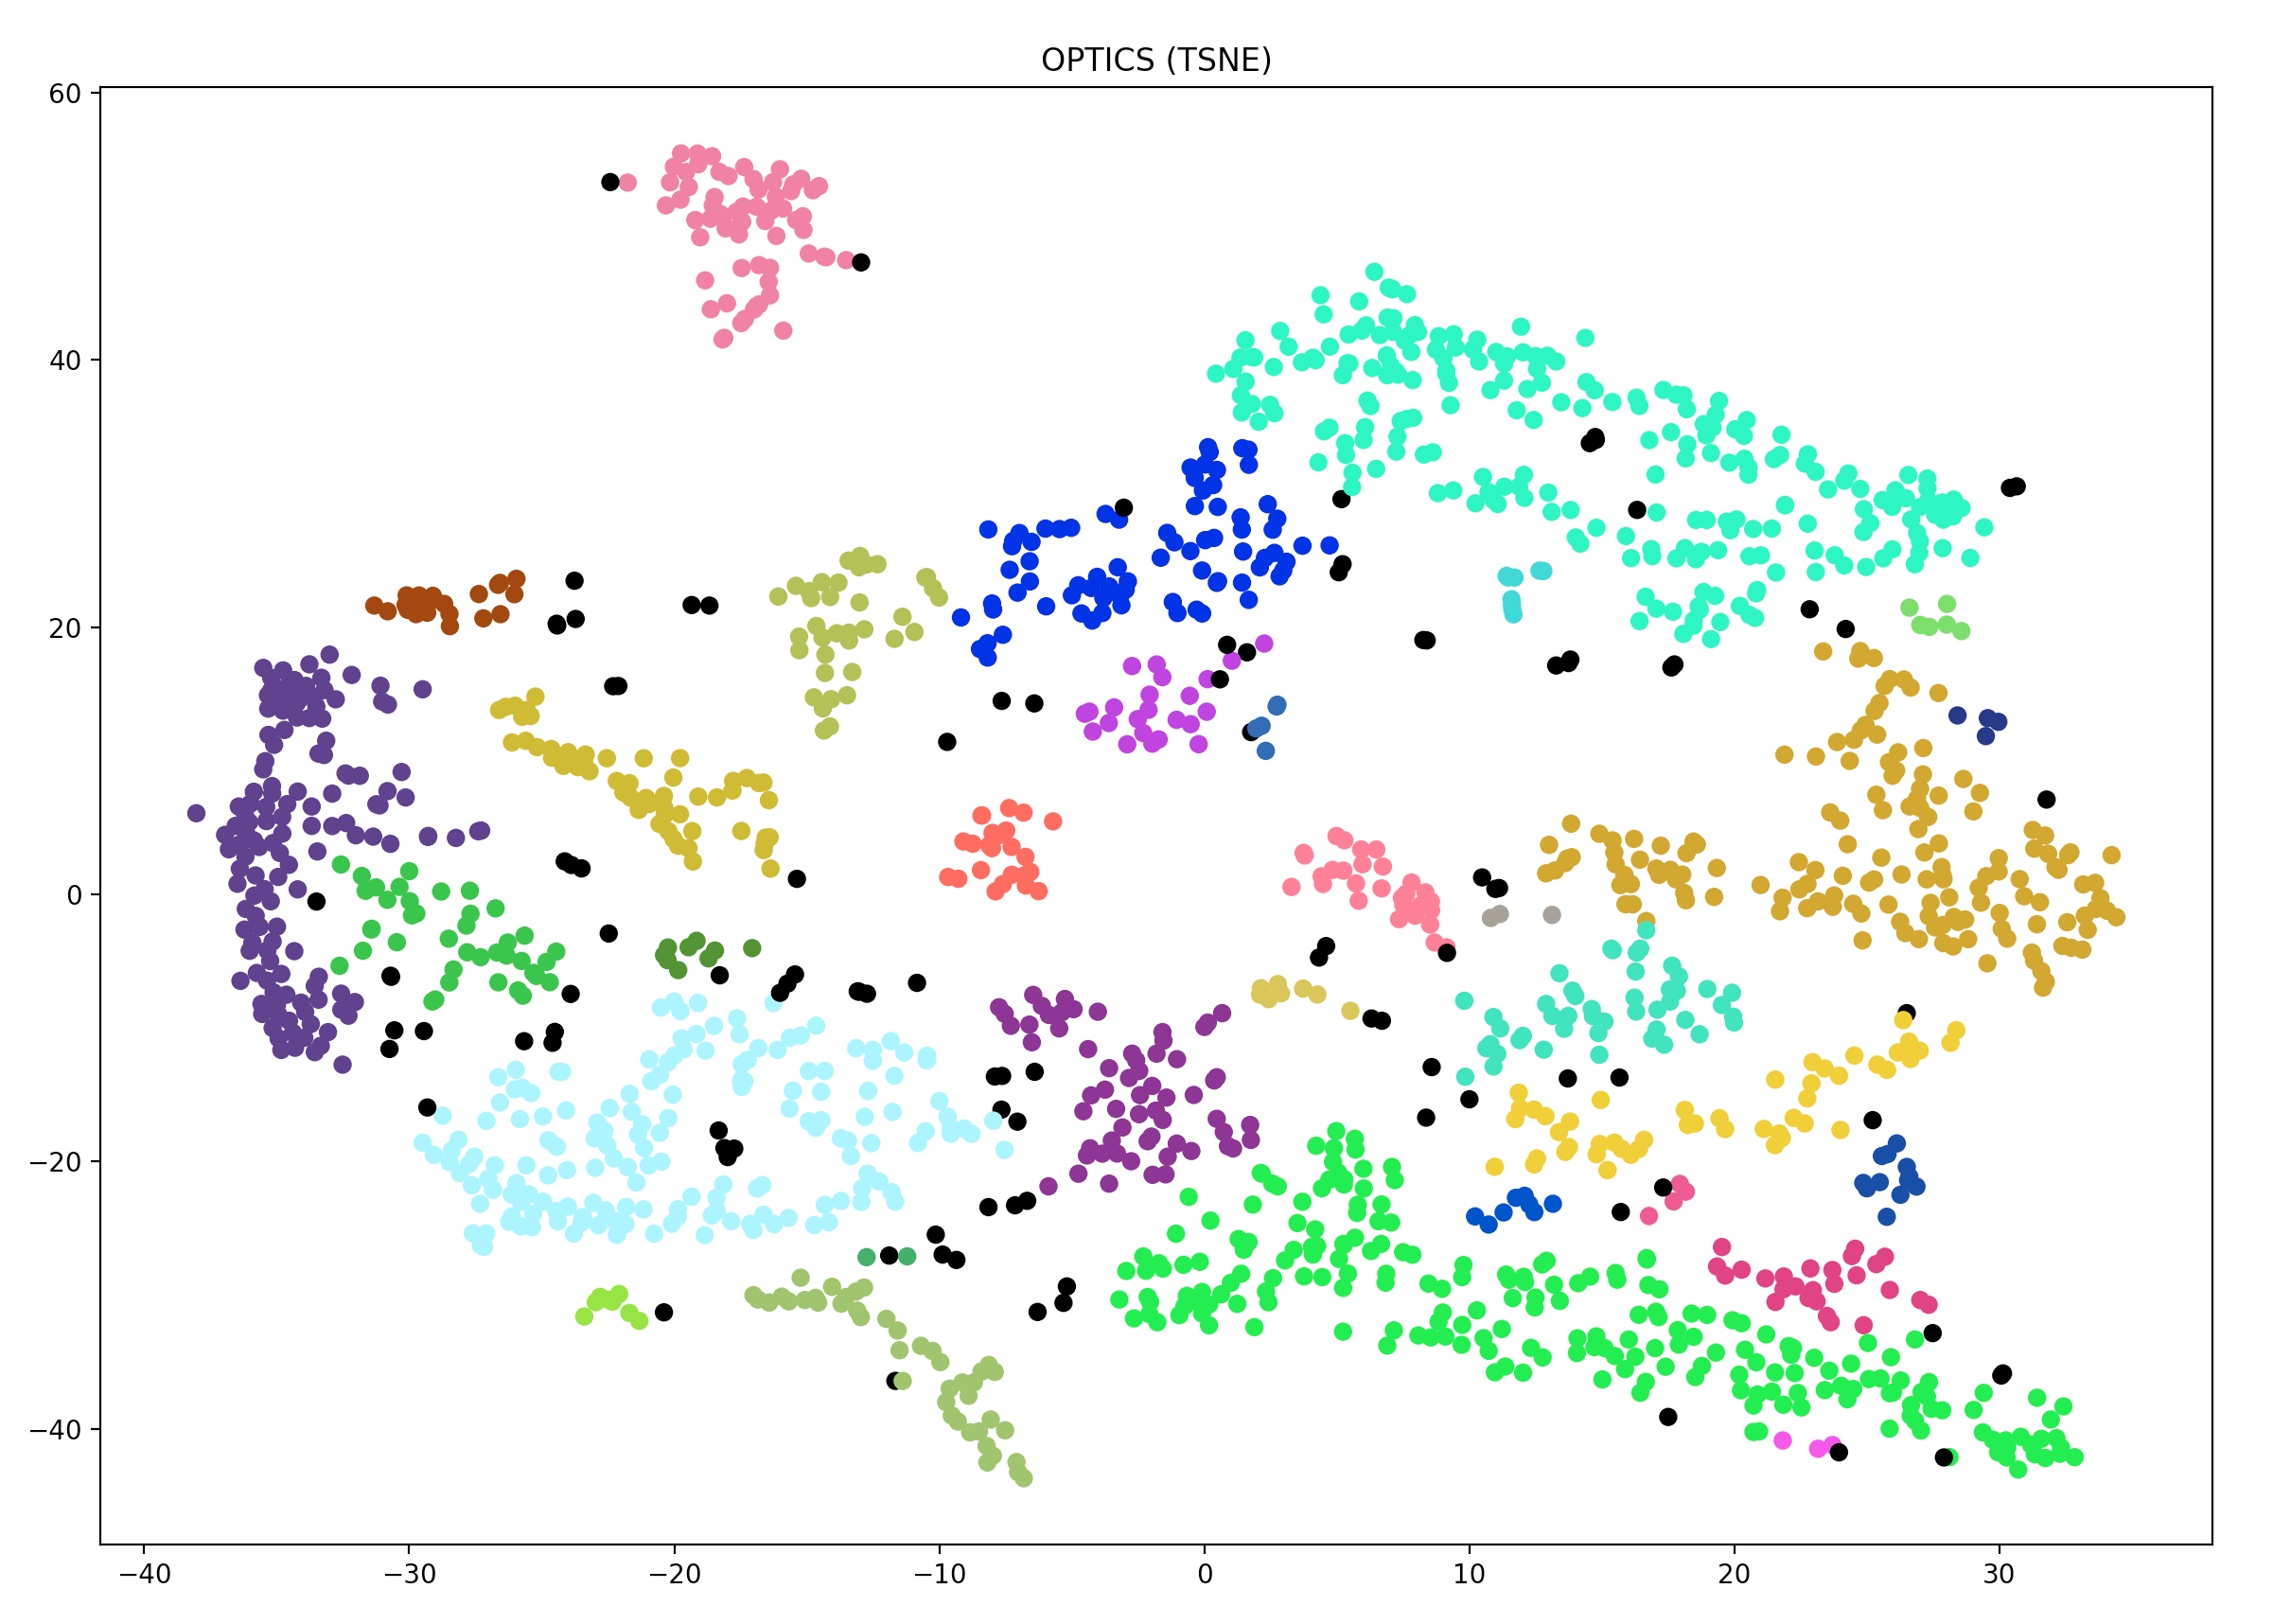
\includegraphics[width=1\textwidth]{./images/OPTICS/1h-1-OPTICS-DBSCAN.png}
  \caption{1h dataset OPTICS clustering (first column - 15 min), using DBSCAN clustering.}
  \end{subfigure}%
  \hfill
  \begin{subfigure}{.5\textwidth}\captionsetup{width=.8\linewidth}
    \centering
    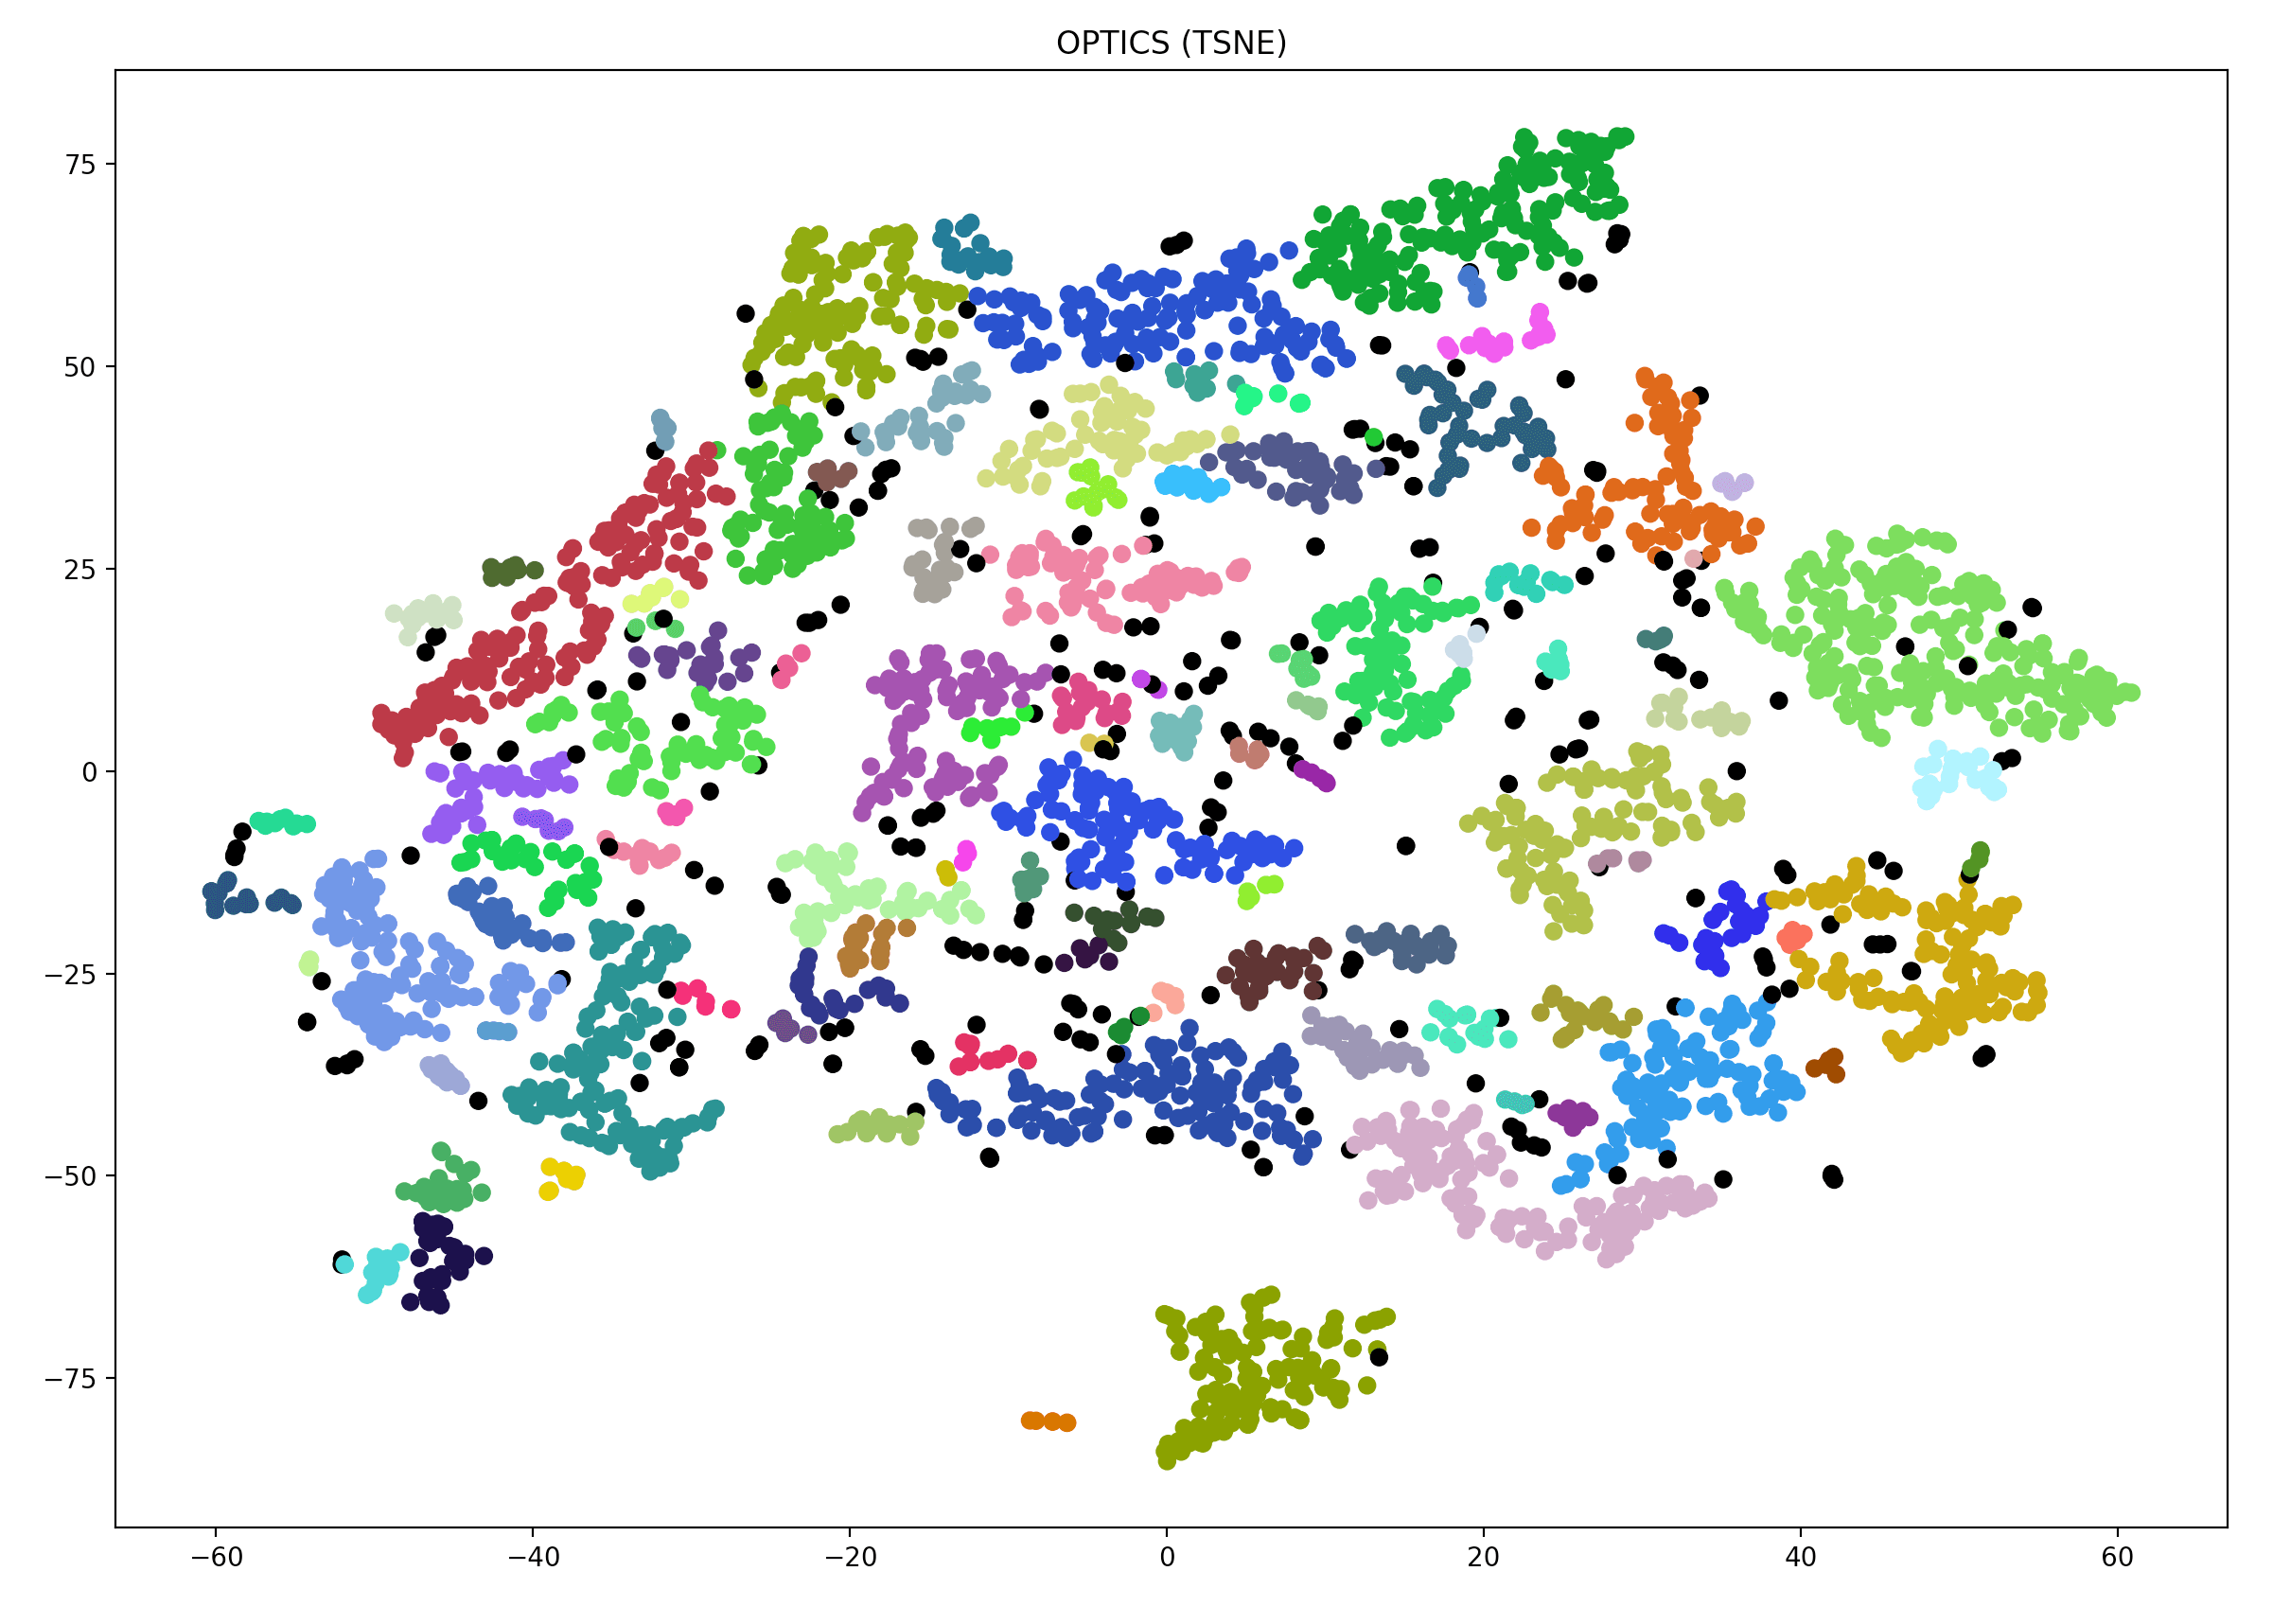
\includegraphics[width=1\textwidth]{./images/OPTICS/3h-1-OPTICS-DBSCAN.png}
    \caption{3h dataset OPTICS clustering (first column - 30 min), using DBSCAN clustering.}
  \end{subfigure}
  \caption{}
  \label{figure:OPTICSResults}
  \end{figure}

\begin{figure}[H]
  \centering
  \begin{subfigure}{.5\textwidth}\captionsetup{width=.8\linewidth}
    \centering
    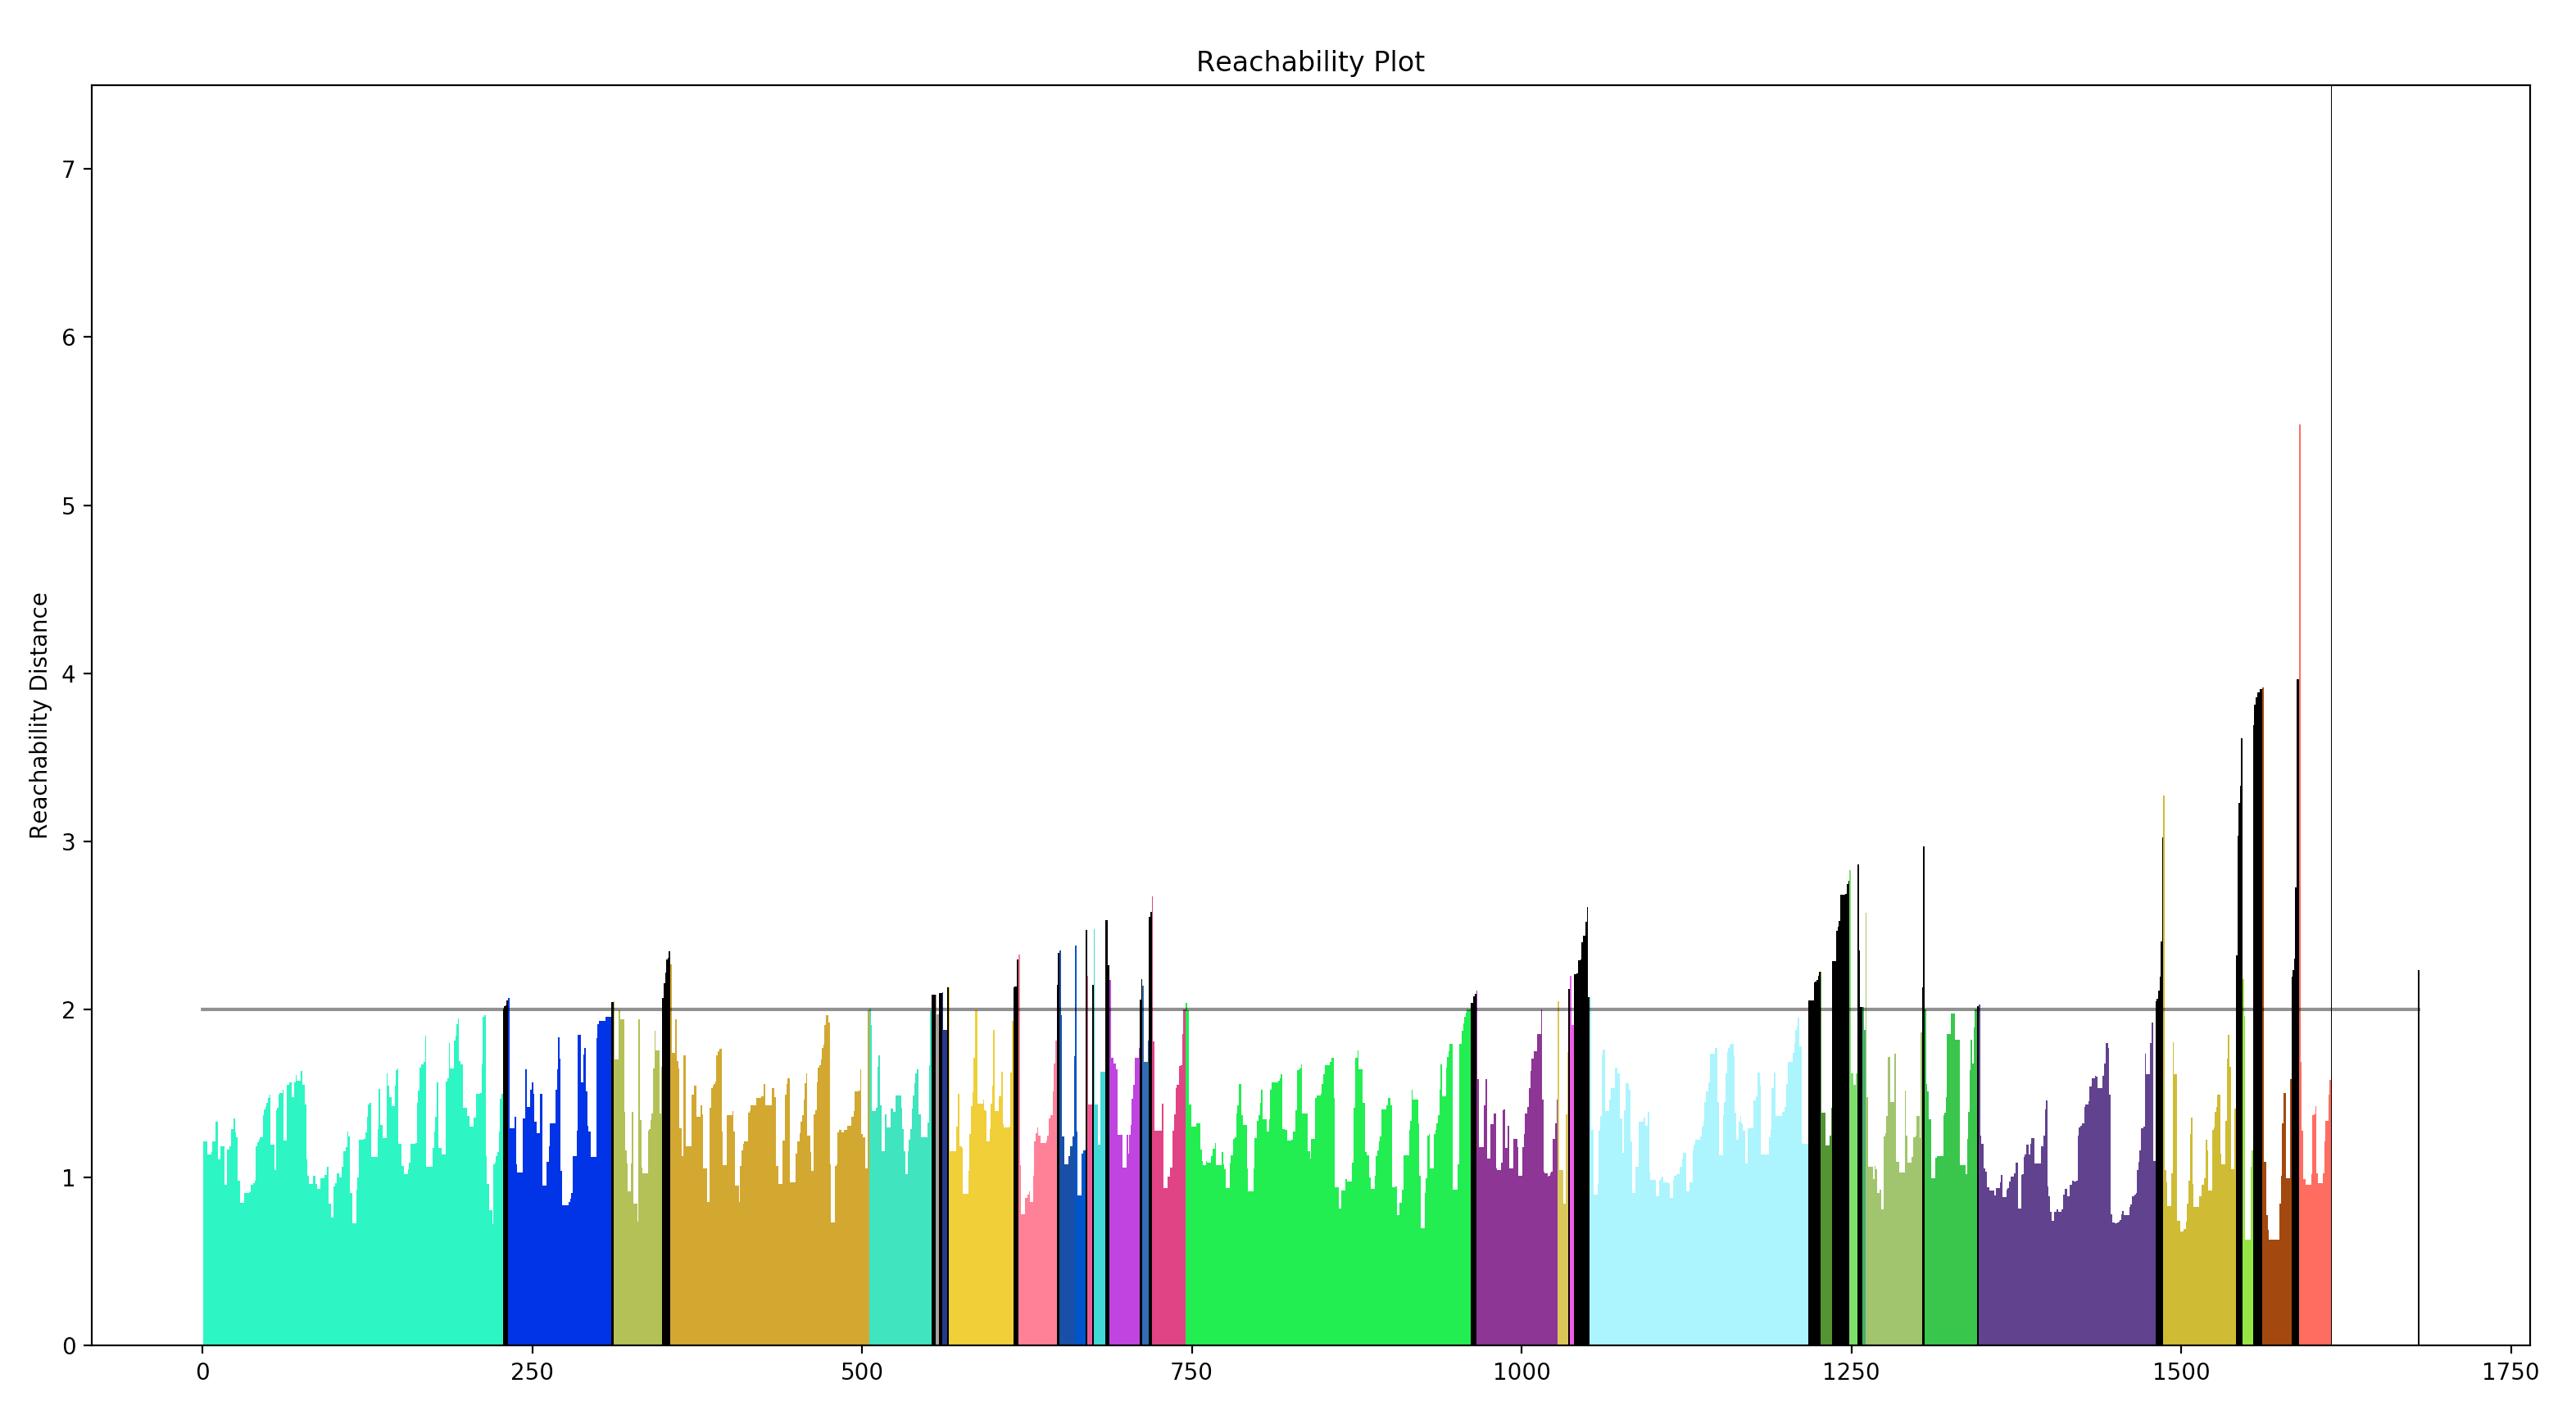
\includegraphics[width=1\textwidth]{./images/OPTICS/1h-1-reachabilityPlot-DBSCAN.png}
  \caption{1h dataset OPTICS reachability plot (first column - 15 min), using DBSCAN clustering.}
  \end{subfigure}%
  \hfill
  \begin{subfigure}{.5\textwidth}\captionsetup{width=.8\linewidth}
    \centering
    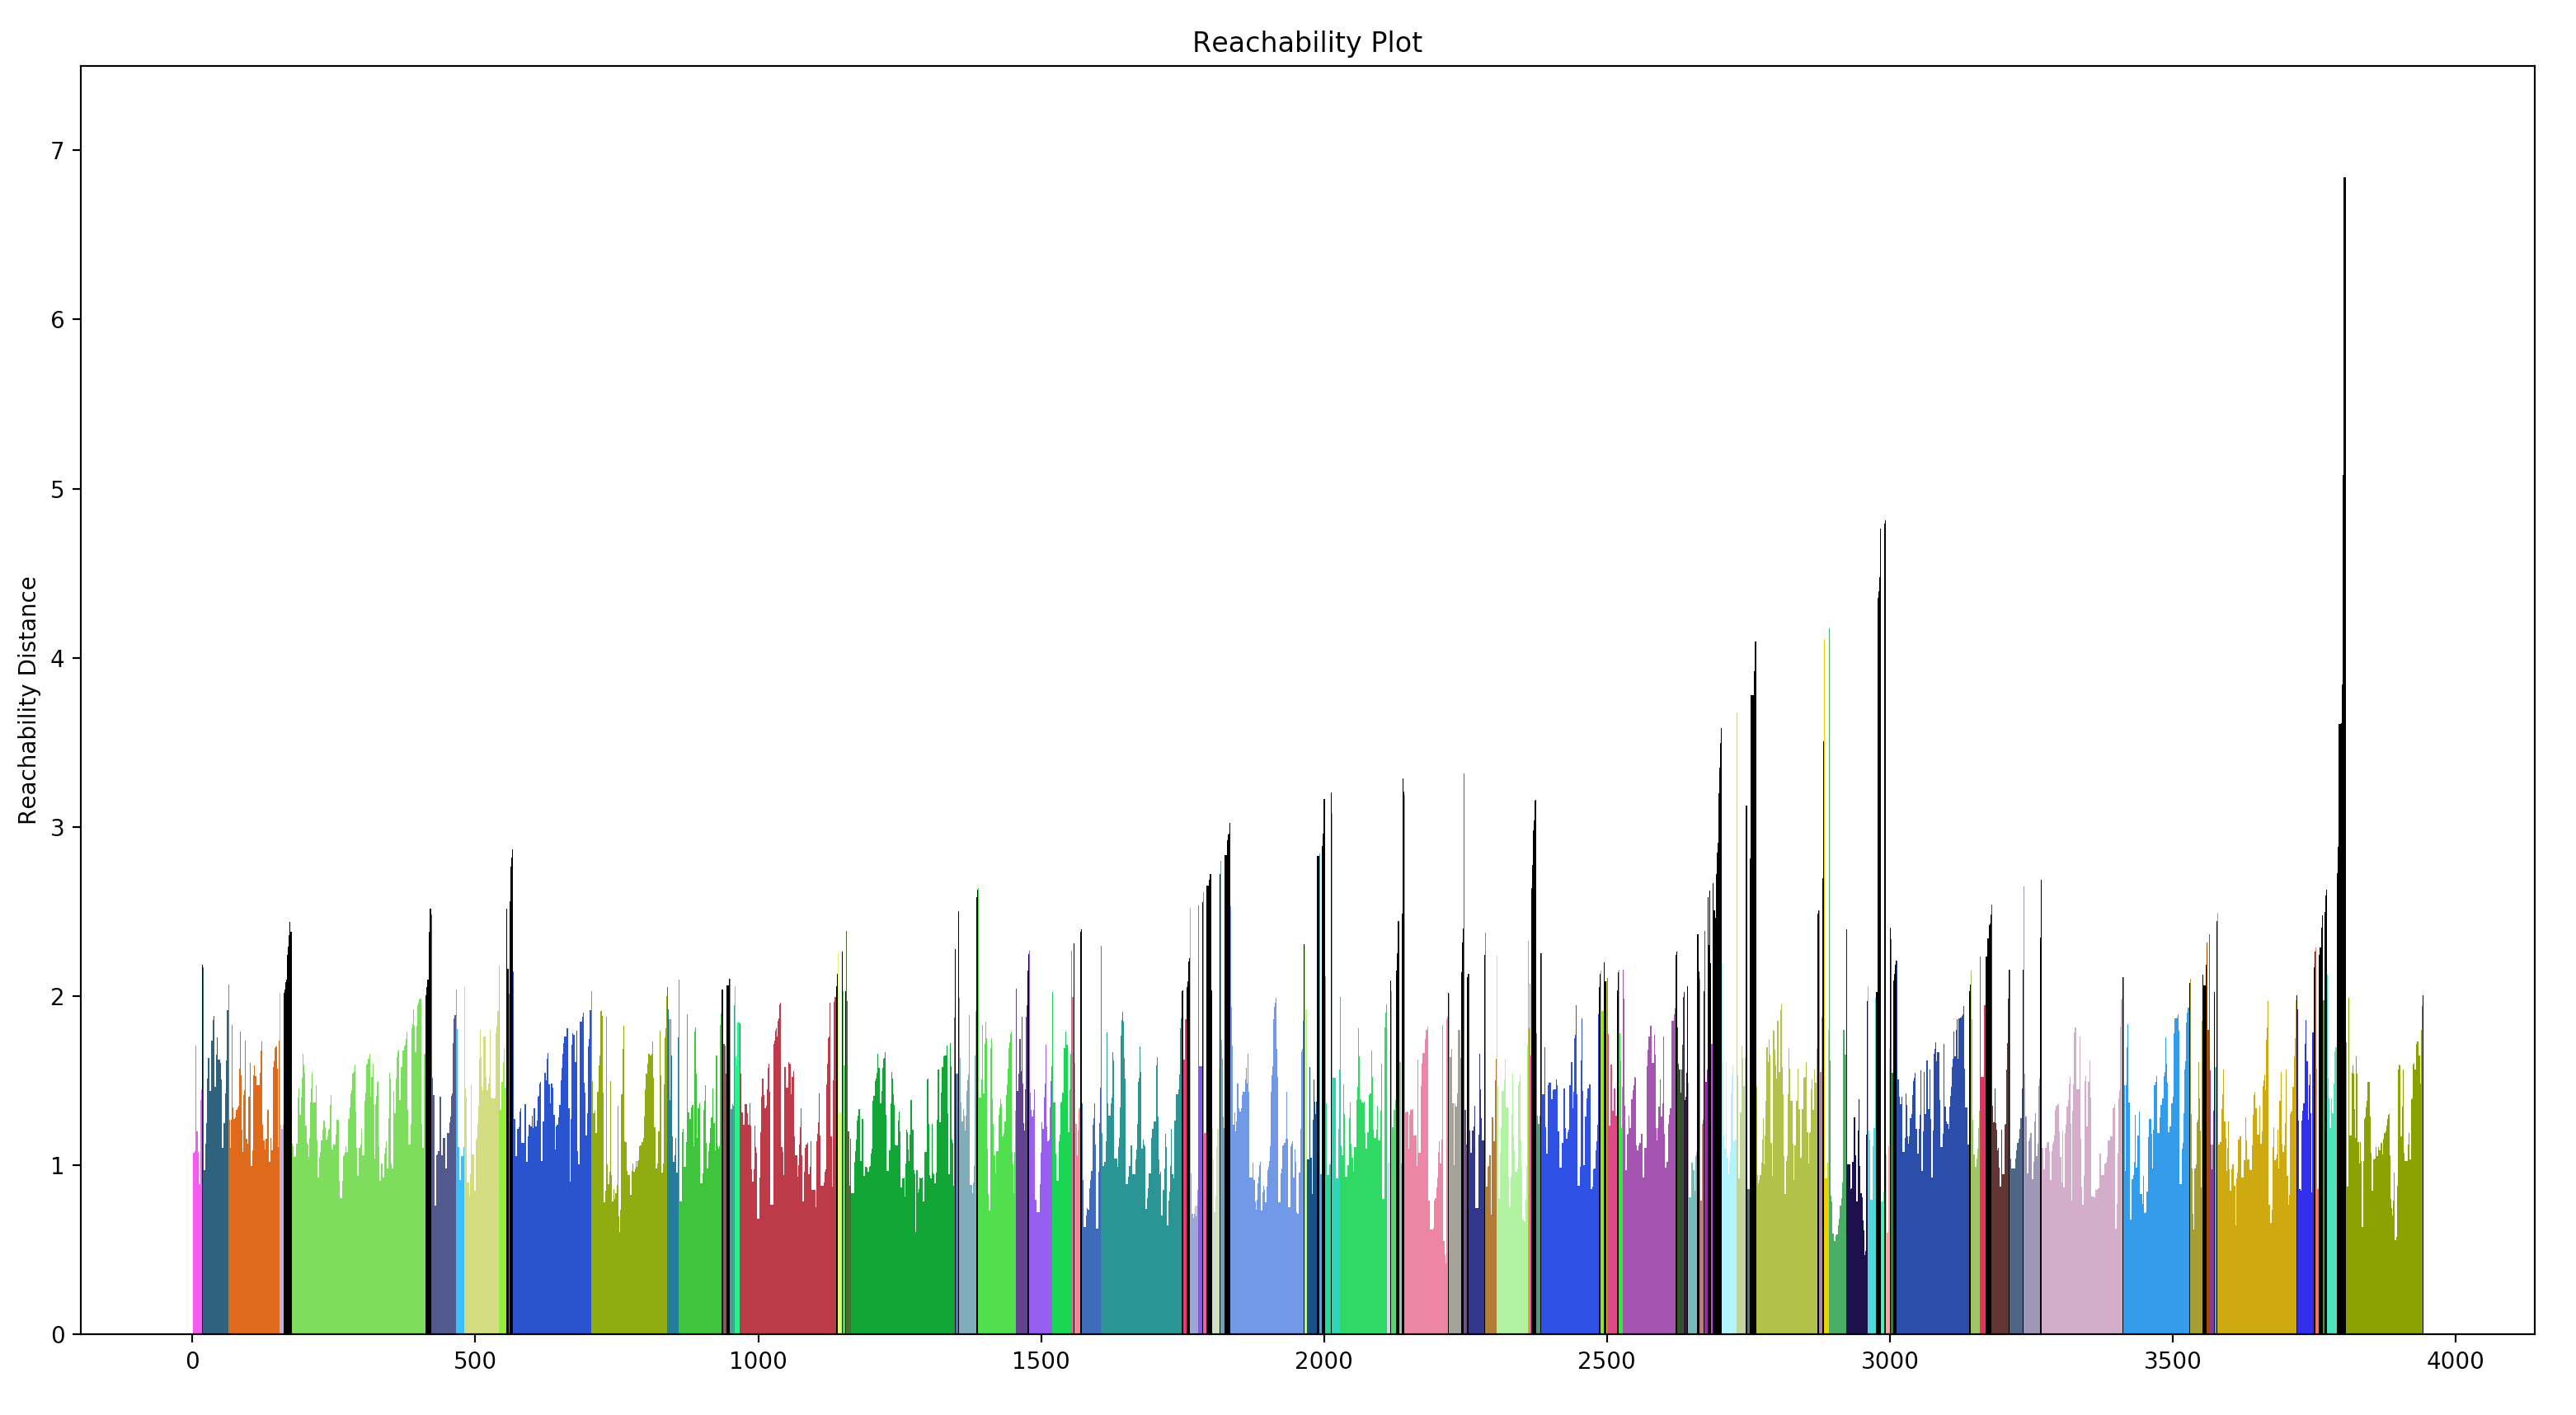
\includegraphics[width=1\textwidth]{./images/OPTICS/3h-1-reachabilityPlot-DBSCAN.png}
    \caption{3h dataset OPTICS reachability plot (first column - 30 min), using DBSCAN clustering.}
  \end{subfigure}
  \caption{}
  \label{figure:OPTICSResultsReachabilityPlot}
  \end{figure}


The final DBSCAN and OPTICS clusterings scatter plots for each time delta are compared in appendix \ref{appendix:clusteringResults}.
